\documentclass[a4paper,12pt]{book}
\usepackage{graphicx}
\usepackage{natbib}
\usepackage{amsmath}
\usepackage{amsfonts}
\usepackage{float}
\usepackage{caption}
\usepackage{wasysym}

\begin{document}
\begin{center}

\title{Discontinuous Galerkin method for direct numerical simulation of the Navier Stokes equation: Master Thesis Report}


\author{Nirav Vasant Shah, \\M.Sc. Candidate, Water Resources Engineering and Management, \\University of Stuttgart, \\Stuttgart, Deutschland (Germany)\\ 
\and Supervisor: Prof. Dr. Bernard Haasdonk,\\ Institute of Applied Analysis and Numerical Simulation, \\Universitity of Stuttgart,\\ Stuttgart, Deutschland (Germany)\\ \and Co-advisor: Prof. Gianluigi Rozza,\\ Scuola Internazionale Superiore di Studi Avanzati, \\Trieste, Italy \\ \and Co-advisor: Dr. Martin Hess,\\ Scuola Internazionale Superiore di Studi Avanzati, \\Trieste, Italy }
\date{\today}
\maketitle

\end{center}

\tableofcontents

\newenvironment{spmatrix}[1]
 {\def\mysubscript{#1}\mathop\bgroup\begin{pmatrix}}
 {\end{pmatrix}\egroup_{\textstyle\mathstrut\mysubscript}}

\chapter{Introduction}

The topic of the thesis deals with the numerical solution of Navier Stokes equation which is the core of Computational Fluid Dynamics. The thesis performs numerical simulation of the Navier Stokes equation through the Discontinuous Galerkin method.

The goal of the thesis is to derive, discretize and implement the Discontinuous Galerkin weak form of Navier Stokes equation and perform numerical simulation of the Navier Stokes equation. In the course of the numerical solution we measure the simulation efforts.

In chapter 2, Navier Stokes equation is introduced. We first derive the Navier Stokes equation from the conservation equation or Reynolds Transport Theoreom. We discuss the flow classification and important issues related to numerical simulation of the Navier Stokes equation. At the end of the chapter we discuss boundary conditions and its consequences on well posedness of the problem.

In Chapter 3, we bring the problem from a continuous domain to a finite domain by introducing discretisation. We first introduce grid, constituents of elements and transformation between local and global geometry. Further the function spaces over the grid are discussed during which, the basis function or Ansatz function, different function spaces for pressure and velocity are discussed. We further introduce and discuss the weak form of the Navier Stokes equation, discrete form of the Navier Stokes equation with boundary condition and properties of weak form.

In Chapter 4, we discuss the implementation of the discrete form of the Navier Stokes equation in RBmatlab, an opensource software developed at the University of Stuttgart and the University of M\"unster, for numerical simulation. During the chapter we discuss basis function formation in RBmatlab, matrix assembly, dimension of assembled matrices and boundary condition implementation.

In Chapter 5, we present results from numerical experiments, analyze results from benachmark problems, discuss used solvers and newton method for non linear iteration.

In the appendix, supplementary theoretical background is provided which is expected to help the readers to better comprehend the thesis.

As future development, the equation can be parametrized for parameters such as fluid properties, geometry of domain or boundary conditions. This allows the approximation of the numerical solution, with approximation being with respect to parameter space. The solution of the parametrized form can be stored for reduced basis evaluations.

If the Proper Orthogonal Decomposition is introduced, it sorts and segregates the stored snapshots, solution at a parameter, based on eigen value. This sorted and segregated snapshots with parametrised form can be used for prediction of full numerical solution. In this process the evaluations are made faster but with increase in approximation error. We compare the time saving vs. induced error.

\chapter{Engineering perspective and mathematical formulation} 

The subject of mathematical applications in fluid mechanics starts with  one of the variants of the Navier Stokes equation. Almost all processes of fluid mechanics require considerations related to the Navier Stokes equation. Hence the importance of Navier Stokes equation is impossible to be ignored as far as mathematical approaches in fluid mechanics are concerned. The numerical method for the incompressible equation is far more simple as compared to the compressible Navier Stokes equation. This is due to removal of dependence on the equation of state. 

\section{Derivation of Navier Stokes equation}\cite{white}

Before deriving the Navier Stokes equation we introduce some notations. The domain is denoted by $\Omega \subseteq \mathbb{R}^d $. The domain boundary is denoted by $\partial \Omega$. The domain boundary is divided into Dirichlet boundary $\Gamma_D$ and Neumann boundary $\Gamma_N$ i.e. $\Gamma_D \cup \Gamma_N = \partial \Omega $. 

The governing equations for the incompressible Navier Stokes flow are conservation equations: Mass conservation and Momentum conservation. The conservation equations are derived based on the concept of control volume and control surface. The control volume is the volume, fixed or moving with constant velocity in space, through which the fluid moves. The control surface is the surface enclosing the control volume. All equations can be derived from Reynold's transport equation:\cite{white}


\begin{equation} \label{rtt} 
\frac{dB'}{dt'}|_{cs} = \frac{d}{dt'} \int_{cv} b' \rho dV + \int_{cs} b' \rho u.dA 
\end{equation}

\begin{center}
$cv$ = Control volume\\
$cs$ = Control surface\\
$B'$ = Extensive property under consideration  \\
$b'$ = Intensive property corresponding to B \\
$\rho$ = Density of fluid \\
$u$ = Velocity of fluid\\
\end{center}

If in the above equation $B'$ is substituted as momentum $P$, correspondingly $b'$ as velocity $u$, we obtain the change in momentum which as per Newton's Second law of Motion is equal to the sum of external forces acting on the system. 

\begin{equation}\label{External force lhs}
F = \frac{dP}{dt'} = \frac{d}{dt'} \int_{cv} u \rho dV + \int_{cs} u \rho u.dA 
\end{equation}

This sum of forces arises from stresses $\sigma$ (shear stresses and normal stresses) and external force $f$ such as weight. 

\begin{equation}\label{External force rhs}
F = \int_{cs} \sigma \cdot dA + \int_{cv} \rho f dV
\end{equation}
\\
$\sigma =$ Stress\\
$f =$ External force per unit volume\\

Equating external force with change in momentum i.e. equating \eqref{External force lhs} and \eqref{External force rhs} and with the application of Gauss divergence theorem we derive the Navier Stokes equation.

\begin{equation} \label{navier_stokes}
-2\nabla \cdot (\nu \nabla^s u) + (1/\rho) \nabla p + (u \cdot \nabla)u = f \quad   \textnormal{in}  \quad \Omega
\end{equation} 

The incompressible mass conservation equation can be written as
\begin{equation}\label{mass_conservation}
\nabla \cdot u=0 \quad   \textnormal{in}  \quad \Omega \quad \textrm{.}
\end{equation}

The boundary conditions can be expressed as,

Dirichlet boundary:
\begin{equation}\label{dirichlet_ns}
u=u_D \quad \textnormal{on} \quad \Gamma_D
\end{equation}

Neumann boundary:
\begin{equation} \label{neumann_ns}
-pn + 2\nu(n \cdot \nabla^s)u = t \quad   \textnormal{on}  \quad \Gamma_N
\end{equation}

Where,\\
$u$ = flow velocity and $u:\Omega \rightarrow \mathbb{R}^d$ \\
$p$ = pressure and $p:\Omega \rightarrow \mathbb{R}$\\
$\nu$ = kinematic viscocity (fluid property) $\nu:\Omega \rightarrow \mathbb{R}$\\ 
$\rho$ = density (fluid property) $\rho:\Omega \rightarrow \mathbb{R}$\\
$f$ = external force $f:\Omega \rightarrow \mathbb{R}^d$\\
$u_D$ = specified flow velocity at Dirichlet boundary $u_D:\partial \Omega_D \rightarrow \mathbb{R}^d$\\
$n$ = normal unit vector $n:\partial \Omega \rightarrow \mathbb{R}^d$\\
$t$ = specified Neumann flux $t:\Gamma_N \rightarrow \mathbb{R}^d$\\
$\nabla^s = \frac{1}{2}(\nabla + \nabla^T)$\\


The equation \eqref{navier_stokes} is known as Strong form.

It can be seen that the steady state Navier Stokes equation is non linear and has two unknown variables, pressure $p$ and velocity $u$. The additional equation added by continuity equation is hence necessary in order to obtain a sufficient number of equations for the number of unknowns.

We also introduce the dimensionless number Reynolds number, $Re$ which is the most characteristic quantity of the flow. The Reynolds number is defined as the ratio of Inertial force to the viscous force,

\begin{equation} \label{reynolds_number}
Re =  u L / \nu
\end{equation}

Where, $L$ is the Characteristic geometrical dimension, for example the diameter of a pipe in case of pipe flow or the span of the wing of an aircraft in case of flow over an aircraft wing.\\

\subsection{Direct numerical simulation} 

We now differentiate between the type of flows, Laminar and Turbulent.\\
A Laminar flow is characterised by well defined velocity and pressure field and low Reynolds number. This flow has very low velocity and pressure fluctuations. The viscous force is balanced by the pressure force and the flow has negligible inertial force. Mathematically, the non linear term in \eqref{navier_stokes} is no longer present. This equation is known as Stokes equation.\cite{white}\\

The strong form of Stokes equation is as follow,

\begin{equation} \label{stokes_strong_form}
-\nu \Delta u + \nabla p = f \quad \textrm{in} \quad \Omega
\end{equation}

\begin{equation} \label{dirichlet condition stokes}
u = u_D \quad \textrm{on} \quad \Gamma_D
\end{equation}

\begin{equation} \label{neumann condition stokes}
-pn + \nu n \cdot \nabla u = t \quad \textrm{on} \quad \Gamma_N
\end{equation}
\\

In contrast, the Turbulent flow is characterised by fluctuations in velocity and pressure field and a high Reynolds number. The flow has high velocity and an inertial force is present in addition to a viscous and a pressure force. This inertial force makes the Equation \eqref{navier_stokes} non linear. The fluctuations of velocity and pressure are of the order of the Kolmogrov scale.\\

The method used for solving Equation \eqref{navier_stokes} numerically is known as Direct Numerical Simulation, abbreviated as DNS. The direct numerical simulation could be computationally very expensive especially in applications such as turbulent flows as the time and space grid size is of the order of the Kolmogrov scale but the time period or space dimension over which the simulation is carried out are very large. In order to avoid such computational expenses alternate models are used replacing the original model. However, the alternate model can not explain completely the flow physics. The prediction of accurate flow physics description requires economical numerical solution of \eqref{navier_stokes}. It is to be noted that simulation of turbulent flow is always a compromise between required flow physics prediction and computational efforts.

\section{Wellposedness of strong form of Navier Stokes equation}

\chapter{Discretization and function spaces}
\section{Grid geometry}

In numerical anlysis the problem is solved on finite domain. This domain is constructed by projecting original domain onto a subdomain called as grid. If the original domain is denoted by $\Omega$ we denote the grid by $\mathcal{T}$. In the present case we use triangular grid and denote each triangle as $\tau_k$. We also note that $\Omega_h = \cup_{k=1}^{nel} \tau_k$ where $nel$ is the total number of elements in the grid. Each triangle is an 'Element' of the grid. The boundary betwen elements i.e. interelement boundary is denoted by $\Gamma$. In case of a grid, the boundaries comprise of domain boundaries and interelement boundaries i.e. $\partial \Omega_h = \Gamma_D \cup \Gamma_N \cup \Gamma$. During discussion on jump operator and average we denote the element under consideration as $\tau_{h}^-$ and neighbouring element as $\tau_{h}^+$. \begin{Huge}
Add photo here of neighbouring and self element to clarify notation
\end{Huge}. We also denote the normal pointing from element itself towards neighbouring element as $n^+$ and the normal pointing from neighbouring element towards element itself as $n^-$. Corresspondingly every quantity on element itself is denoted by superscript $+$ and from neighbouring element is denoted by $-$.  We denote by $h_{\tau_k}$ the diameter of element on grid $\tau_k$ such that $h_{\tau_k} = \sup ||x-y||$ where, $(x,y) \in \tau_k$. We also denote by $\theta$ the smallest angle of element $\tau$ in the grid $\mathcal{T}$.

In case of a 2-dimensional domain the grid could be a triangular grid or a rectangular grid. The triangular grids are useful for irregular geometry and also on regular geometry if flow physics, and correspondigly the solution, is expected to be complex. This flexibility requires additional efforts to define the grid accurately. That is, unlike a structured grid, an unstructured grid needs to define connectivity of vertices, which form an edge, which in turn forms a face. These faces in case of 3-dimensional grid constitute a tetrahedral elements. In case of a 2-dimensional grids we have only faces which are 2-dimensional entity, edges which are 1-dimensional entities and points or vertices which are 0-dimensional entities.

For triangular grids we also consider a Barycentric co-ordinate system. In Barycentric co-ordinate system any point within the triangle is represented in terms of vertices forming the triangle. Any point $r$ within a triangle is expressed in terms of vertices $r_1,r_2,r_3$ forming the triangle. This is represented as,

\begin{equation}\label{barycentric point}
r = \lambda_1 r_1 + \lambda_2 r_2 + \lambda_3 r_3
\end{equation}

where, $\lambda_1, \lambda_2, \lambda_3$ are weights. The weights satisfy the criterion,

\begin{equation}\label{lambda constraint}
\lambda_1 + \lambda_2 + \lambda_3 = 1
\end{equation}

Hence, we only need to specify 2 values in 2-dimensional plane in order to fully define the position of point.

For example, the centroid of triangle will have $\lambda_1 = 1/3, \lambda_2 = 1/3$. By equation \eqref{lambda constraint} we have $\lambda_3=1/3$.

\section{Grid parameters}

We refer to "Grid parameters" as the geometrical parmeters which are dependent only on the geometry of the problem or the grid or both. These parameters do not depend upon the mathematical formulation but are supplementry to the mathematical formulation. On the triangular grid we have 3 entities faces, edges, vertices as explained above. From faces we have the area (equivalent to volume of element in case of a 3-dimensional grid) and the Jacobian. As explained later in the weak form of the Navier Stokes Discontinuous Galerkin and transformation between local and global geometry the area of element is useful for volume intergral terms and the Jacobian is useful for gradient transformation. From edges we derive the edge length $l$ which is useful for boundary integral terms and normal vector $n$ which is useful for flux calculation. The normal vector is the unit vector normal to the boundary pointing outward from the element. Every element has 3 neighbouring element and the element shares each of his edge with one of its neighbour. From vertices we derive the vertex index which helps to define the connectivity of the vertices which is useful especially in case of unstructured grid. 

In order to give clear visualization of domain or precisely, the continuous domain and the grid or discretized domain we introduce a unit square with circular obstacle with the center of the circle coinciding with center of square. 

\newpage

\begin{figure}
  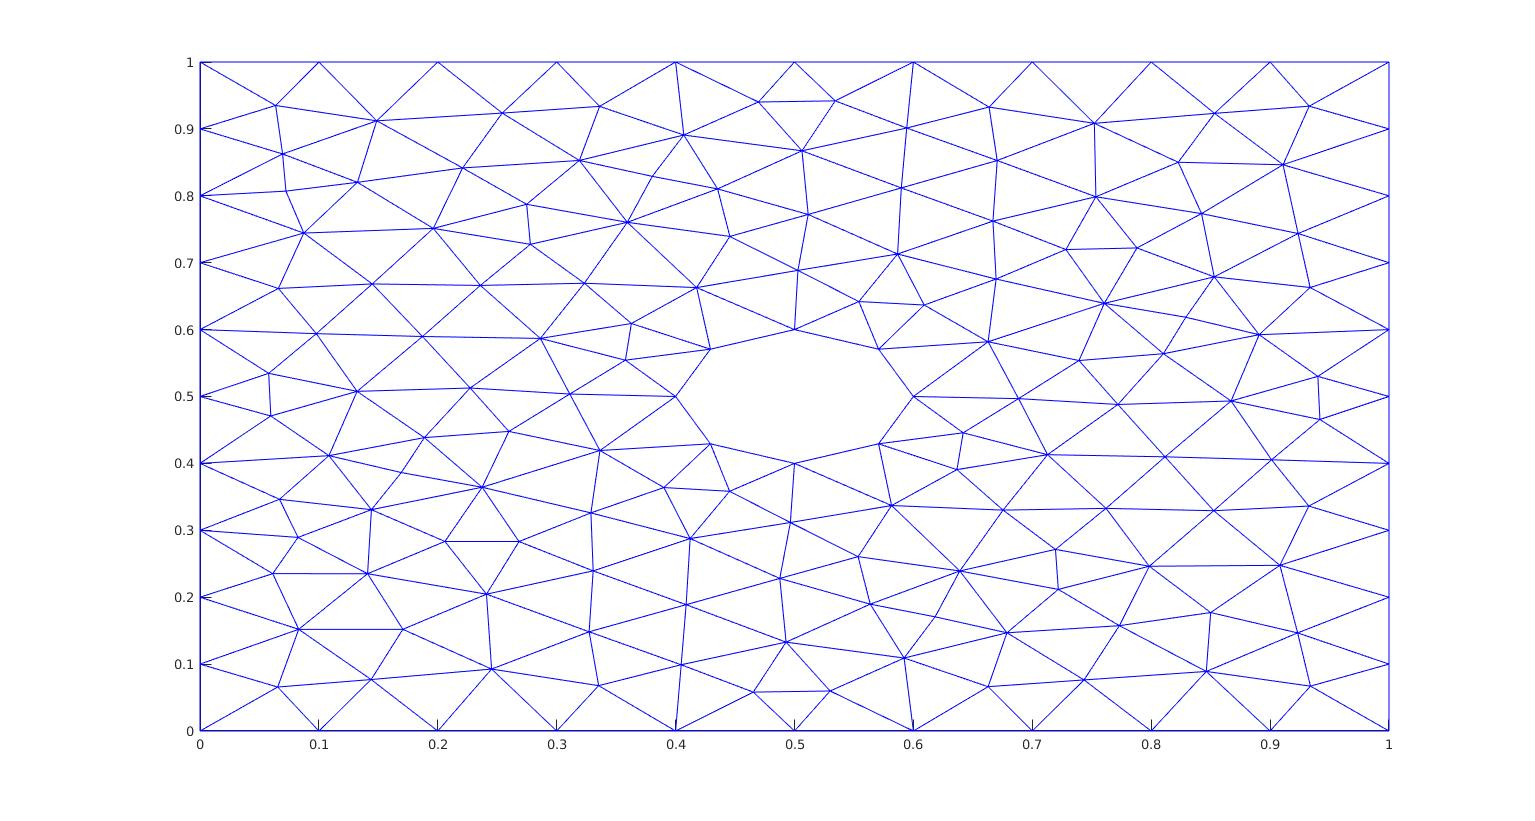
\includegraphics[width=\linewidth,scale=0.5]{grid.jpg}
  \caption{Discretized domain or grid}
  \label{fig:Mesh}
\end{figure}

\begin{figure}
  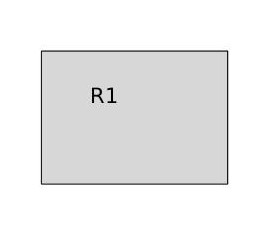
\includegraphics[width=\linewidth,scale=0.5]{domain.jpg}
  \caption{Continuous domain}
  \label{fig:Domain}
\end{figure}

\section{Discontinuous Galerkin Method}

In the context of the discontinuous Galerkin method we introduce the function spaces $V_h$($\mathcal{T}$) and $Q_h$($\mathcal{T}$) for analytical solution of velocity and analytical solution of pressure respectively. The space containing high fidelity solution (in this case Discontinuous Galerkin) is called truth space denoted by $V_h$ for velocity and $Q_h$ for pressure. The dimension of truth space is denoted as $N_h$. (The subscript $h$ hereafter refers to the truth space.)

\begin{equation} \label{velocity_test}
V_h = \lbrace \phi \in (L^2(\Omega))^2| \phi |_\tau \in P^D(\tau) \forall \tau \in \mathcal{T} \rbrace
\end{equation}

\begin{equation} \label{pressure_test}
Q_h = \lbrace \psi \in L^2(\Omega)| \psi |_\tau \in P^{D-1}(\tau) \forall \tau \in \mathcal{T} \rbrace
\end{equation}

Here, $P^D(\tau)$ denotes space of polynomials of degree at most $D$ over $\tau$.

We apply a similar procedure as in the finite element method i.e. multiplying the partial differential equation by a test function and integration by parts. However, we note that our test function is not continuous on the interface. Hence, we require flux approximations and jumps at the interface. These requirements have given rise to different discontinuous Galerkin methods. For explanation of each method we refer to literatures such as \cite{persson} for local discontinuous Galerkin and \cite{Montlaur} for the Compact discontinuous Galerkin and the Interior penalty method. 

Discontinuous Galerkin methods for the Navier Stokes equation were compared by \cite{Montlaur}. The local discontinuous Galerkin (LDG) method extends the computational stencil beyond immediate neighbours whereas compact discontinuous Galerkin (CDG) and interior penalty method (IPM) only connect to neighbouring elements. The CDG method provides more flexibility with respect to the stabilisation constant (citation needed) at the cost of additional simulation effort related to computation of the lifting operator, while the IPM method requires restrictions on penalty parameter in order to maintain coercivity of bilinear form. Both methods, CDG and IPM, have almost similar convergence rates. 

\section{Nodal basis function and Orthonormal basis function}

The "Basis functions" are also known as "Ansatz function". There are two kinds of basis function which are used in the application of Finite element or Discontinuous Galerkin Method. 
Before, explaining the difference between two types of basis functions, we understand the procedure to define the function completely. \\

In order to define a polynomial of given degree completely, we need to calculate its co-efficients. A polynomial of degree $n$ in a 1-dimensional domain has $n+1$ coefficients. In case of a 2-dimensional domain the number of coefficients become $(n+1)(n+2)/2$. To define these coefficients the known values of function at a number of points equal to the number of coefficients is required. These points are known as nodes. In case of triangular element, the nodes are located as,\\

1. For polynomials of degree 1 i.e. $D=1$, the nodes are selected as vertices of an element.\\
2. For polynomials of degree 2 i.e. $D=2$, the nodes are selected as the vertices of an element and mid points of edges.\\

\begin{figure}
  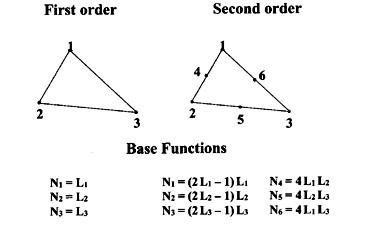
\includegraphics[width=\linewidth]{fem_triangle.jpg}
  \caption{Finite Element nodes on triangle for $D=1$ and $D=2$ \cite{plasma}}
  \label{fig:Nodes on Triangular Element}
\end{figure}

Similarly for higher order polynomials the nodes are selected as shown in Figure \ref{fig:Nodes on Triangular Element}.

\begin{figure}
  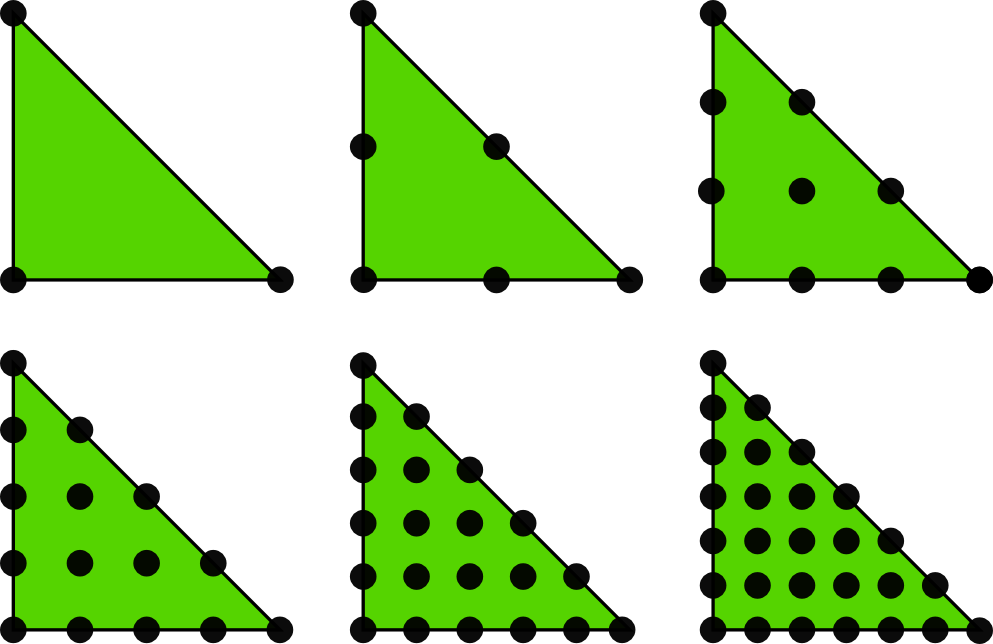
\includegraphics[width=\linewidth]{fem_triangle_2.png}
  \caption{Finite Element nodes on triangle for polynomials of different degrees \\ http://hplgit.github.io/INF5620/doc/pub/sphinx-fem/.\_main\_fem009.html}
  \label{fig:Nodes on Triangular Element}
\end{figure}

\subsection{Nodal Basis Functions}

Nodal basis functions are also known as "Shape function". Such a basis function has value of 1 at its respective node and 0 at other nodes. At all other points it is approximated based on the degree of the basis function. 

\subsection{Orthonormal Basis Functions}

Orthonormal basis functions are the basis functions defined in such a way that all basis functions are orthonormal to each other. The number of orthonormal basis functions for a given element is the same as the number of nodal basis functions. In fact, in present analysis the orthonormal basis functions are derived from Nodal basis functions.

\section{Global and local co-ordinate system}

Integral terms are evaluated on a reference triangle instead of the element itself. Accordingly, a co-ordinate transformation is performed for every element from a reference triangle for evaluating integrals. The co-ordinate system in which the reference triangle lies is called reference or local co-ordinate system and the co-ordinate system in which element itself lies is called global co-ordinate system. The reference triangle has vertices $(0,0),(1,0),(0,1) \in \mathbb{R}^2$ in order. The element is defined by vertex indices in order forming triangle. The mapping from reference triangle $\hat{T}$ to each element $\tau_k$ is defined by the mapping,

\begin{equation}\label{local global mapping}
F_k:\hat{T} \mapsto \tau_k
\end{equation}

This mapping function is defined as,

\begin{equation}\label{local global mapping equation}
F_k: X = J_k \hat{X} + C
\end{equation}

Here,
\\
$J_k$ = Jacobian matrix of element $\tau_k$ for transformation from local co-ordinate system to global co-ordinate system, $J_k \in R^{d \times d}$\\
$C$ = Translational vector for transformation from local co-ordinate system to global co-ordinate system, $C \in R^d$\\
$X$ = Co-ordinates of points of element in Global co-ordinate system, $X \in \tau_k$ \\
$\hat{X}$ = Co-ordinates of points of reference triangle in local co-ordinate system, $\hat{X} \in \hat{T}$\\

We represent the image of a global function space or grid constituent on reference triangle by superscript $\hat{•}$ . This function space is known as local basis function space. 

\begin{picture}(300,100)(0,0) 
\put(0,0){\line(1,0){50}}
\put(50,0){\line(1,1){100}}
\put(0,0){\line(3,2){150}}
\put(200,0){\line(1,0){100}}
\put(300,0){\line(-1,1){100}}
\put(200,100){\line(0,-1){100}}
\end{picture}

\begin{center}
Global geometry (left) to Local geometry (right)
\end{center}

The volume integral of a function $g(x)$ in global coordinates is related to volume integral on reference geometry as 
\begin{equation}\label{integral_local_global_volume}
\int_\Omega g(x) dx = \sum_{k=1}^{nel} \int_{\tau_k} g(x) dx = \sum_{k=1}^{nel} \int_{\hat{T}} g(\hat{x}) |\det(J_k)| d \hat{x}
\end{equation}

The linear boundary integral of a function $g(x)$ on global coordinates is related to boundary integral on reference geometry as, 
\begin{equation}\label{integral_local_global_boundary}
\int_{\Gamma} g(x) ds = \int_{\hat{\Gamma}} g(\hat{x}) ld \hat{s}
\end{equation}

Also, the following holds,
\begin{equation}\label{derivative_transformation}
\nabla g = JIT_k \quad \hat{\nabla} \hat{g} 
\end{equation}


where,
\\
$l$ = length of boundary on global geometry\\
$g$  = A function in global co-ordinate system, $g:\Omega \mapsto \mathbb{R}$\\
$\hat{g}$  = A function in local co-ordinate system corresponding to function in $g$ in global coordinate system, $\hat{g}:\hat{T} \mapsto \mathbb{R}$\\
$JIT_k$ = $J_k^{-1}$, Jacobian inverse transpose of element k

Here $g$ and $\hat{g}$ satisfy,
\begin{equation}\label{func_transformation}
g(x) = \hat{g}(\hat{x}) \quad \textrm{for}  \quad x = F_k(\hat{x}) \quad \textrm{according to equation \eqref{local global mapping equation}}
\end{equation}

\section{Jump operator}

The jump operator of a quantity $[u]$ at an internal boundary is defined as,
\begin{equation}\label{jump operator}
[u]=u^+ \cdot n^+ + u^- \cdot n^-
\end{equation}

where $n$ is the unit normal to the element boundary pointing outwards from the element.

As pointed out by \cite{Montlaur2} this jump definition has two disadvantages.

1. The function space of the quantity itself and the function space of the jump are diferrent that is, the jump of a vector is scalar and jump of a scalar is vector.\\
2. The use of this definition camouflages the presence of a normal.\\

To overcome this disadvantages \cite{Montlaur2} used the jump definitions as ,

1. \\
$[[pn]] = p^+ n^+ + p^- n^- $ on $\Gamma$\\
$[[pn]] = p n $ on $\Gamma_D$\\
where $p$ is scalar. \\

2. \\
$[[n \otimes v]] = n^+ \otimes v^+ + n^- \otimes v^-$ on $\Gamma$\\
$[[n \otimes v]] = n \otimes v$ on $\Gamma_D$\\
 or \\
$[[n \cdot v]] = n^+ \cdot v^+ + n^- \cdot v^-$ on $\Gamma$\\
$[[n \cdot v]] = n \cdot v$ on $\Gamma_D$\\
where $v$ is vector and ($n \otimes v = v n^T$)\\

\section{Average operator}

Similarly the average operator is defined as,

\begin{equation}\label{average operator}
\left\lbrace u \right\rbrace = \frac{u^+ + u^-}{2}  
\end{equation} 

\section{$L^2$ scalar product}

We denote the scalar product by $(p,q)$ which refers to,

If $p$ and $q$ are scalars,
\begin{equation}\label{inner product scalars}
(p,q)=\int_{\Omega} pq d \Omega 
\end{equation}

If $p$ and $q$ are vectors,
\begin{equation}\label{Inner product vectors}
(p,q)=\int_{\Omega} p \cdot q d\Omega
\end{equation}

If $p$ and $q$ are tensors,
\begin{equation}\label{Inner product tensors}
(p,q)=\int_{\Omega} p:q d\Omega
\end{equation}

\section{Problem statement}

With the above background we are now ready to derive weak formulation and define problem in weak form. Following the approach presented by \cite{Montlaur} and \cite{Montlaur2} we arrive at weak form of Stokes and Navier Stokes interior penalty approximation.

\subsection{Stokes strong, weak and discrete form} \label{Stokes_flow_ch3}

The strong form of Stokes equation is as follow,

\begin{equation} \label{stokes_strong_form_ch3}
-\nu \Delta u + \nabla p = f \quad \textrm{in} \quad \Omega
\end{equation}

\begin{equation} \label{dirichlet condition stokes_ch3}
u = u_D \quad \textrm{on} \quad \Gamma_D
\end{equation}

\begin{equation} \label{neumann condition stokes_ch3}
-pn + \nu n \cdot \nabla u = t \quad \textrm{on} \quad \Gamma_N
\end{equation}

The weak form of Stokes equation is as follow,

\begin{equation}\label{stokes_weak_ch3}
\begin{split}
a_{IP}(u,\phi) + b(\phi,p) + (\{p\},[n\cdot \phi])_{\Gamma \cup \Gamma_D} = l_{IP}(\phi) 
\end{split}
\end{equation}
\\
\begin{equation}
\begin{split}
a_{IP}(u,\phi) = (\nabla u, \nabla \phi) + C_{11} ([n \otimes u],[n \otimes \phi])_{\Gamma \cup \Gamma_D} \\
- \nu (\{\nabla u\},[n \otimes \phi])_{\Gamma \cup \Gamma_D} - \nu ([n \otimes u],\{\nabla \phi\})_{\Gamma \cup \Gamma_D}
\end{split}
\end{equation}
\\

It is to be noted that penalty paramter $C_{11}$ is to be kept large enough to maintain coercivity of bilinear form.\\

\begin{equation}
\begin{split}
l_{IP}(\phi) = (f,\phi) + (t,\phi)_{\Gamma_N} + C_{11} (u_D,\phi)_{\Gamma_D} - (n \otimes u_D, \nu \nabla \phi)_{\Gamma_D}
\end{split}
\end{equation}

The discrete form of Stokes equation is written as,

\begin{equation} \label{stokes discrete_ch3}
AU + BP = F_1 \textrm{.}
\end{equation}

The strong form of continuity equation is as follow,

\begin{equation}
\nabla \cdot u = 0 \quad \textrm{in} \quad \Omega \textrm{.}
\end{equation}

and the weak for of continuity equation is as follow,

\begin{equation}\label{contiuity_weak_ch3}
\begin{split}
b(u,\psi) + (\{\psi\},[n\cdot u])_{\Gamma \cup \Gamma_D} = (q,n\cdot u_D)_{\Gamma_D} \textrm{.}
\end{split}
\end{equation}

The discrete form of continuity equation is written as,

\begin{equation} \label{continuity discrete_ch3}
B^T U  = F_2 \textrm{.}
\end{equation}

Discrete form of equations can be written in Matrix form as, 

\begin{equation} \label{Stokes_matrix_ch3}
\begin{spmatrix}{K}
    A & B \\
    B^T & 0
\end{spmatrix}
\begin{spmatrix}{X}
    U \\
    P
\end{spmatrix}
=
\begin{spmatrix}{B}
    F_1  \\
    F_2
\end{spmatrix}
\end{equation}

Here, $b(\phi,\psi) = -\int_{\Omega} \psi \nabla \cdot \phi$, $(\cdot , \cdot)$ is $L^2$ inner product, $\{\cdot\}$ is average operator, $[\cdot]$ is jump operator. 

\subsection{Upwinding} \label{upwinding}

Upwinding is method used to discretise the convective term. In case of discontinuous Galerkin method we define the upwinding as follow.\\

If $n_\tau$ is the unit normal from $\tau_1$ to $\tau_2$ and if we denote the upwind value of function $w$ as $w^{up}$ \cite{riviere}
\begin{equation}
\begin{split}
w^{up} = w|_{\tau_1} \quad \textrm{if} \quad w \cdot n_\tau \geq 0 \\
w^{up} = w|_{\tau_2} \quad \textrm{if} \quad w \cdot n_\tau < 0
\end{split}
\end{equation}
\\
In our analysis this is explicitly defined in the term $c(u,u,\phi)$ in section \ref{n_s_ch3}. The scheme is such that,
\begin{equation}
\begin{split}
u^{up} = u \quad \textrm{if} \quad u \cdot n \geq 0 \\
u^{up} = u^{ext} \quad \textrm{if} \quad u \cdot n < 0
\end{split}
\end{equation}

\subsection{Navier Stokes strong, weak and discrete form:} \label{n_s_ch3}

Stokes flow is an example of Navier Stokes flow with low Reynolds number, $Re$. In case of high Reynolds number the inertial force can no longer be neglected and hence we need to add inertial foces in Stokes flow. 

The strong form of Navier Stokes equation can be written as,

\begin{equation} \label{navier_stokes_strong_ch3}
-\nu \Delta u + \nabla p + (u \cdot \nabla) u = f \quad \textrm{in} \quad \Omega
\end{equation}

with Dirichlet and Neumann boundary condition as per section \ref{Stokes_flow_ch3}. Also the continuity equation as mentioned in section \ref{Stokes_flow_ch3} is valid.

The inertial forces term in weak form with upwinding (section \ref{upwinding}) is as below,

\begin{equation}
\begin{split}
c(w;u,\phi) = \sum_{i=1}^{nel} \int_{\partial \Omega_i \setminus \Gamma_N} \frac{1}{2} [[(w \cdot n_i)(u^{ext} + u) - |w \cdot n_i|(u^{ext} - u)]] \cdot \phi \\ + \int_{\Gamma_N} (w\cdot n) u \cdot \phi -((w\cdot \nabla)\phi,u)
\end{split}
\end{equation}

Hence, Navier Stokes equation can be written as,

\begin{equation}\label{navier_stokes_weak_ch3}
\begin{split}
a_{IP}(u,\phi) + c(u;u,\phi) + b(\phi,p) + (\{p\},[n\cdot \phi])_{\Gamma \cup \Gamma_D} = l_{IP}(\phi) 
\end{split}
\end{equation}

Here, we can see that the $c(u,u,\phi)$ is non linear term.

In discrete form this equation can be written as,

\begin{equation}
AU + C(U) U + BP = F
\end{equation} 

Here, $C(U)$ is a matrix which is dependent on solution vector $U$ and hence making the system of equation non linear.

In matrix form the Navier Stokes equation with Continuity equation can be written as,

\begin{equation} \label{Stokes_matrix_ch3}
\begin{spmatrix}{K}
    A+C(U) & B \\
    B^T & 0
\end{spmatrix}
\begin{spmatrix}{X}
    U \\
    P
\end{spmatrix}
=
\begin{spmatrix}{B}
    F_1  \\
    F_2
\end{spmatrix}
\end{equation}

In the present analysis, we use Newton method to solve non linear system of equations. We present the Newton scheme in section \ref{newton_method}. 

Our problem statement now reduces to, find $(u,p) \in (\mathbb{V},\mathbb{Q})$ such that $\forall (\phi,\psi) \in (\mathbb{V},\mathbb{Q})$ equation \ref{stokes_weak_ch3} for Stokes flow and \ref{navier_stokes_weak_ch3} for Navier Stokes flow is satisfied.

\subsection{Boundary condition}

We impose in our analysis boundary condition weakly. This is done by the rhs terms $(t,\phi)_{\Gamma_N}$, $(u_D,\phi)_{\Gamma_D}$, $(n \otimes u_D, \nu \nabla \phi)_{\Gamma_D}$.

\chapter{Implementation aspects} \label{implementation_aspects}

We discuss now the implementation of discrete formulation of Navier Stokes discontinuous Galerkin weak formulation in RBmatlab, A MATLAB library containing all our reduced simulation approaches for linear and nonlinear, affine or arbitrarily parameter dependent evolution problems with finite element, finite volume or local discontinuous Galerkin discretizations. 

Before we discuss details of implementation it is important to understand some frequently used terminologies and the data type of Basis Function and derivative of basis function in RBmatlab.

\section{Terminologies}


A. $params$ and $paramsP$ : $params$ and $paramsP$ are structures corressponding to velocity and pressure respectively and primarily containing following fields\\

1. $dimrange$ : We refer $dimrange$ as dimension of range or solution. In present analysis this means Velocity has $dimrange$ of 2 and Pressure has $dimrange$ of 1.\\

2. $pdeg$ : We refer $pdeg$ as the degree of polynomial used as interpolation polynomial.\\

3. $ndofs\_per\_element$ : We refer $ndofs\_per\_element$ as the number of degrees of freedom over an element. \\

4. $dofs$ : $dofs$ is the field containing solution vector.

5. $ndofs$ : $ndofs$ is the total number of degrees of freedom.

6. $show\_sparsity$ : $show\_sparsity$ is the switch for plotting sparsity pattern.

B. $grid$ : $grid$ is the structure containing following fields\\

7. $nelements$ : $nelements$ is total number of elements in grid.\\

8. $NBI$ : $NBI(i,j)$ represents element number of $j$th neighbour of element $i$. 1$\leq i \leq nelements$ and 1$\leq j \leq$3.\\

9. $NX$ and $NY$ : $NX(i,j)$ and $NY(i,j)$ represent x component and y component of normal from  element $i$ to $j$ numbered neighbour.\\

10. $JIT$ : $[JIT(k,:,1)',JIT(k,:,2)']$ represents Jacobian Inverse Transpose of element $k$.\\

11. $A$ : $A(k)$ represents area of $k$th element.\\

12. $EL$ : $EL(i,j)$ represents length of edge between element $i$ and $j$th neighbour of Element $i$. The notation $EL$ is used when $i$ refers to superscript $+$ and $j$ refers to element with superscript $-$.\\

We also use some other local variables as below:

13. $k$ : $k$ represents the element number and 1$\leq k \leq nelements$.\\

14. $ids$ : $ids(i,:)$ represents the indices of degree of freedom of element $i$ where 1$\leq i \leq nelements$ in global degree of fredom vector. Size of $ids(i,:)$ is $ndofs\_per\_element$. $ids\_velocity$ corressponds to indices corressponding to velocity and $ids\_pressure$ corressponds to indices corressponding to pressure. Further notations such as $ids\_velocity\_neighbour$ should be read as $ids$ of velocity degree of freedom of neighbouring element. $ids$ are generated by routine $ldg\_global\_dof\_index$.\\

\section{Basis Function in RBmatlab}

The Basis functions in RBmatlab is generated by routine called $ldg\_evaluate\_basis.m$.\\

We approximatete the solution at any point from solution of degrees of freedom in orthonormal basis. In matrix formulation this means basis function is matrix of the size,

\begin{equation}\label{basis_func_rbmatlab}
\phi_h \epsilon \mathbb{R}^{ndofs\_per\_element X dimrange}
\end{equation}

where each row of $\phi_h$ denotes one degree of freedom.

This representation creates many zeros in matrix, however, it does not require new evaluation for each component of vector quantity in $dimrange$ of solution.

Due to the zeros in the basis function, zeros in derivative of basis functions are produced. 

The derivative of basis function is generated by routine $ldg\_evaluate\_basis\_derivative$. The derivative of basis function $(\phi_h)_{i}$, where $1 \leq i \leq nodfs\_per\_element$ is a cell containing matrix $\nabla (\phi_h)_{i}$ of size,
\begin{equation}\label{basis_func_derivative_rbmatlab}
\nabla (\phi_h)_{i} \epsilon \mathbb{R}^{{dimrange} X 2}
\end{equation}

where the colmuns of matrix corresspond to $\nabla_x (\phi_h)_{i}$ and $\nabla_y (\phi_h)_{i}$ .

\section{Assembly of average operator}

Average of quantity, $A_h$ in discrete form is assembled as,

\begin{equation}\label{Average operator}
{A_h} = (A_h^+ + A_h^-)/2
\end{equation}

The assembly of average operator is relatively simple as compared to jump operator which is explained in section \ref{Jump operator}

\section{Assembly of jump operator} \label{Jump operator}

Jump of quantity, $A_h$ in discrete form is assembled as,
\begin{equation} \label{Jump_operator}
[A_h] = A_h^+ n^+ + A_h^- n^-
\end{equation}

In case of terms such as $[A_h],[B_h]$ we assemble matrices as, 

For internal edges $\Gamma$,

\begin{equation} \label{Jump operator L2}
[A_h],[B_h] = A_h^+ n^+ B_h^+ n^+ + A_h^+ n^+ B_h^- n^- + A_h^- n^- B_h^+ n^+ + A_h^- n^- B_h^- n^-
\end{equation}

and for dirichlet edges $\Gamma_D$

\begin{equation} \label{Jump operator L2 for dirichlet}
[A_h],[B_h] = A_h^+ n^+ B_h^+ n^+ 
\end{equation}


\section{Matrix assemblies}

We repeat here, for conveniece, again the notations of $L^2$ scalar product from weak form

Here, $(p,q)$ refers to,

If $p$ and $q$ are scalars,
\begin{equation}\label{inner product scalars}
(p,q)=\int_{\Omega} pq d \Omega 
\end{equation}

If $p$ and $q$ are vectors,
\begin{equation}\label{Inner product vectors}
(p,q)=\int_{\Omega} p \cdot q d\Omega
\end{equation}

If $p$ and $q$ are tensors,
\begin{equation}\label{Inner product tensors}
(p,q)=\int_{\Omega} p:q d\Omega
\end{equation}

i.e. (.,.) denotes $L_2$ inner product.

It is to be noted that $\hat{\phi_h}$ is evaluated at local coordinate corresponding to global coordinate in accordance with \ref{func_transformation}.

The matrices from weak form of Navier Stokes equation have been assembled in 3 steps,

1. Evaluating function at vertex of local element and transform to global geometry\\
2. Performing integral of function over local element and transform to global geometry(if not done in step 1)\\
3. Performing a loop over all elements and allocate integral at position in global matrix(for bilinear terms)/global vector(for linear terms) according to index of element degree of freedom in global degree of freedom vector.

We also perform numerical integration over domain $\Omega$ as,

\begin{equation}\label{numerical integration}
\int_{\Omega} f(x) = \Sigma_{i=1}^{nop} f(x_i) w_i
\end{equation}

Where, \\

$x_i$ = Location of function evaluation\\
$w_i$ = Weight at corressponding point\\
$nop$ = Number of points\\

The location of function evaluation, number of points and weights are based on Gaussian quadrature rule.

Also the determinant of jacobian is twice the area of triangle.

\begin{equation}\label{determinant to area}
J(k) = 2A(k)
\end{equation}

With this preliminary informations we discuss now the assembly of matrices.

1. $(\nabla \phi, \nabla \phi)$:\\

Step 1: Evalauation of $(\nabla \phi , \nabla \phi)$,

We first evaluate derivative of $\hat{\phi}$ and $JIT(k,:,:)$ through $ldg\_evaluate\_basis\_derivative$ and grid structure. We also perform elementary operation so as to receive one global basis function in each row. The matrix transformation from local derivative to global derivative is based on the formula \ref{derivative_transformation}.

We than assemble matrix $res_1[i,j]=\phi_i \phi_j^T$ for $1 \leq i,j \leq ndofs\_per\_element$\\

Step 2: Performing integration in global co-ordinate system,

We perform the numerical integration as per \ref{numerical integration} 

$res_2 = \int_{\hat{\Omega}} res_1 2 grid.A(k)  d \hat{\Omega}$\\

Step 3: Looping over each element and performing following operation in each loop $res_3[ids\_velocity,ids\_velocity]=res_2$\\


2. $([n \otimes \phi_h], [n \otimes \phi_h])_{\Gamma \cup \Gamma_D}$ :

Step 1: On local element following functions are evaluated,\\
\\
$res_1^{++} = [n \otimes \hat{\phi_h]}^+ [n \otimes \hat{\phi_h}]^+$\\
$res_1^{+-} = [n \otimes \hat{\phi_h}]^+ [n \otimes \hat{\phi_h}]^-$\\
$res_1^{-+} = [n \otimes \hat{\phi_h}]^- [n \otimes \hat{\phi_h}]^+$\\
$res_1^{--} = [n \otimes \hat{\phi_h}]^- [n \otimes \hat{\phi_h}]^-$\\

Please note that $\hat{\phi_h}$ is evaluated at local coordinate corressponding to global coordinate.

Step 2: In step 2 we perform following integration, 
We perform the numerical integration as per \ref{integral_local_global_boundary}
\\ 
$res_2^{++} = \int_{\Gamma} res_1^{++} grid.EL$\\
$res_2^{+-} = \int_{\Gamma} res_1^{+-} grid.EL$\\
$res_2^{-+} = \int_{\Gamma} res_1^{-+} grid.EL$\\
$res_2^{--} = \int_{\Gamma} res_1^{--} grid.EL$\\

Step 3: Loop over all elements, define the global assembly matrix as zero matrix and perform following operation in each loop,
\\
$res_3^{++}[ids\_velocity\_self,ids\_velocity\_self] = res_2^{++}$\\
$res_3^{+-}[ids\_velocity\_self,ids\_velocity\_neighbour] = res_2^{+-}$\\
$res_3^{-+}[ids\_velocity\_neighbour,ids\_velocity\_self] = res_2^{-+}$\\
$res_3^{--}[ids\_velocity\_neighbour,ids\_velocity\_neighbour] = res_2^{--}$\\

Finally,

$res_3 = res_3^{++} + res_3^{+-} + res_3^{-+} + res_3^{--}$\\

It is to be noted that on dirichlet boundary only $res_1^{++}, res_2^{++}, res_3^{++}$ is evaluated as all other terms are zero.

3. $({\nabla u_h}, [n \otimes \phi_h])_{\Gamma \cup \Gamma_D}$ :

Step 1: On local element following functions are evaluated,\\
\\
$res_1^{++} = {\nabla u_h}^+ [n \otimes \hat{\phi_h}]^+$\\
$res_1^{+-} = {\nabla u_h}^+ [n \otimes \hat{\phi_h}]^-$\\
$res_1^{-+} = {\nabla u_h}^- [n \otimes \hat{\phi_h}]^+$\\
$res_1^{--} = {\nabla u_h}^- [n \otimes \hat{\phi_h}]^-$\\

Step 2: In step 2 we perform following integration, 
We perform the numerical integration as per \ref{integral_local_global_boundary}
\\ 
$res_2^{++} = \int_{\Gamma} res_1^{++} grid.EL$\\
$res_2^{+-} = \int_{\Gamma} res_1^{+-} grid.EL$\\
$res_2^{-+} = \int_{\Gamma} res_1^{-+} grid.EL$\\
$res_2^{--} = \int_{\Gamma} res_1^{--} grid.EL$\\

Step 3: Loop over all elements, define the global assembly matrix as zero matrix and perform following operation in each loop,
\\
$res_3^{++}[ids\_velocity\_self,ids\_velocity\_self] = res_2^{++}$\\
$res_3^{+-}[ids\_velocity\_self,ids\_velocity\_neighbour] = res_2^{+-}$\\
$res_3^{-+}[ids\_velocity\_neighbour,ids\_velocity\_self] = res_2^{-+}$\\
$res_3^{--}[ids\_velocity\_neighbour,ids\_velocity\_neighbour] = res_2^{--}$\\

Finally,

$res_3 = res_3^{++} + res_3^{+-} + res_3^{-+} + res_3^{--}$\\

It is to be noted that on dirichlet boundary only $res_1^{++}, res_2^{++}, res_3^{++}$ is evaluated as all other terms are zero.

The same routine is also used in case of $([n \otimes \phi],{\nabla u})_{\Gamma \cup \Gamma_D}$

4. $({\psi_h}, [n \cdot \phi_h])_{\Gamma \cup \Gamma_D}$ :

Step 1: On local element following functions are evaluated,\\
\\
$res_1^{++} = {\psi_h}^+ [n \cdot \hat{\phi_h}]^+$\\
$res_1^{+-} = {\psi_h}^+ [n \cdot \hat{\phi_h}]^-$\\
$res_1^{-+} = {\psi_h}^- [n \cdot \hat{\phi_h}]^+$\\
$res_1^{--} = {\psi_h}^- [n \cdot \hat{\phi_h}]^-$\\

Please note that $\hat{\phi}$ is evaluated at local coordinate corresponding to global coordinate in accordance with \ref{func_transformation}.

Step 2: In step 2 we perform following integration, 
We perform the numerical integration as per \ref{integral_local_global_boundary}
\\ 
$res_2^{++} = \int_{\Gamma} res_1^{++} grid.EL$\\
$res_2^{+-} = \int_{\Gamma} res_1^{+-} grid.EL$\\
$res_2^{-+} = \int_{\Gamma} res_1^{-+} grid.EL$\\
$res_2^{--} = \int_{\Gamma} res_1^{--} grid.EL$\\

Step 3: Loop over all elements, define the global assembly matrix as zero matrix and perform following operation in each loop,
\\
$res_3^{++}[ids\_velocity\_self,ids\_velocity\_self] = res_2^{++}$\\
$res_3^{+-}[ids\_velocity\_self,ids\_velocity\_neighbour] = res_2^{+-}$\\
$res_3^{-+}[ids\_velocity\_neighbour,ids\_velocity\_self] = res_2^{-+}$\\
$res_3^{--}[ids\_velocity\_neighbour,ids\_velocity\_neighbour] = res_2^{--}$\\

Finally,

$res_3 = res_3^{++} + res_3^{+-} + res_3^{-+} + res_3^{--}$\\

It is to be noted that on dirichlet boundary only $res_1^{++}, res_2^{++}, res_3^{++}$ is evaluated as all other terms are zero.

5. $-\int_{\Omega} \psi \nabla \cdot \phi$
We note that, In accordance with \ref{derivative_transformation}\begin{equation}
\nabla \phi = JIT \hat{\nabla} \hat{\phi}
\end{equation}
and in accordance with \ref{func_transformation}
\begin{equation}
\psi(x) = \hat{\psi} (\hat{x})
\end{equation}

Step 1 : We first evaluate $JIT$, $\hat{\nabla} \hat{\phi}$ and $\psi$ and assemble following local matrix\\
$res_1 = \hat{\psi_i} \hat{\nabla} \cdot \hat{\phi_j}$\\

Step 2 : We integrate the function over domain\\
$res_2 = -\int_{\hat{\Omega}} res_1 2 A(k)$\\

Step 3: Assemble the global matrix\\
$res_3[ids\_presure,ids\_velocity] = res_2$\\

We use the same routine for $-\int_{\Omega} \nabla \cdot \phi_i \psi_j $

6. $(t,\phi)_{\Gamma_N}$:
\\

Step 1: On local element following function is evaluated $res_1=\hat{\phi}_i \cdot t$ in accordance with \ref{func_transformation}\\
Step 2: An integral is performed over an element $res_2=\int_{\Gamma_N} res_1 EL $\\
Step 3: Loop over element having Neumann boundary and perform following operation in each loop $res_3[ids]=res_2$\\

7. $(u_D,\phi)_{\Gamma_D}$:
\\

Step 1: On local element following function is evaluated $res_1=\hat{\phi}_i u_D$ in accordance with \ref{func_transformation}\\
Step 2: An integral is performed over an element $res_2=\int_{\Gamma_D} res_1 EL $\\
Step 3: Loop over element having Dirichlet boundary and perform following operation in each loop $res_3[ids]=res_2$\\

8. $(\psi, n \cdot u_D)_{\Gamma_D} $:

Step 1: On local element following function is evaluated $res_1=\hat{\psi} n\cdot u_D$ in accordance with \ref{func_transformation}\\
Step 2: An integral is performed over an element $res_2=\int_{\Gamma_D} res_1 EL $\\
Step 3: Loop over element having Dirichlet boundary and perform following operation in each loop $res_3[ids]=res_2$\\

9. $(f,\phi) $:

Step 1: On local element following function is evaluated $res_1= \hat{\phi} f$ in accordance with \ref{func_transformation}\\
Step 2: An integral is performed over an element $res_2=\int_{\hat{\Omega}} res_1 2 A(k)$\\
Step 3: Loop over element having Dirichlet boundary and perform following operation in each loop $res_3[ids]=res_2$\\


10. $(n \otimes u_D,\nabla \phi)_{\Gamma_D} $:

Step 1: On local element following function is evaluated $res_1= n \otimes u_D  \nabla \phi$ in accordance with \ref{func_transformation}\\
Step 2: An integral is performed over an element $res_2=\int_{\Gamma_D} res_1 2*A(k)$\\
Step 3: Loop over element having Dirichlet boundary and perform following operation in each loop $res_3[ids]=res_2$\\

We discuss now assembly of non linear terms. We now introduce initial guess $u_k$ whihc will be iterated further.\\

11. $-((u_k \cdot \nabla)\phi , \phi)$:\\
Step 1: On local element following function is evaluated $res_1 = (u_k \cdot \nabla \hat{\phi_i} \hat{\phi_j}) $ in accordance with \ref{func_transformation}\\
Step 2: An integral is performed over an element $res_2= - \int_{\Gamma_D} res_1 EL$\\
Step 3: Loop over all elements and perform following operation in each loop $res_3[ids,ids]=res_2$\\

12. $-((u_k \cdot n)\phi , \phi)$:\\
Step 1: On local element following function is evaluated $res_1 = (u_k \cdot n) \hat{\phi_i} \hat{\phi_j} $ in accordance with \ref{func_transformation}\\
Step 2: An integral is performed over an element $res_2= \int_{\Gamma_N} res_1 EL $\\
Step 3: Loop over all Neumann edge and perform following operation in each loop $res_3[ids,ids]=res_2$\\

13. $((u_k \cdot n)\phi , \phi)$:\\
Step 1: On local element following function is evaluated $res_1 = (u_k \cdot n) \hat{\phi_i} \hat{\phi_j} $ in accordance with \ref{func_transformation}\\
Step 2: An integral is performed over an element $res_2 = \frac{1}{2}  \int_{\Gamma_N} res_1 EL $\\
Step 3: Loop over all Neumann edge and perform following operation in each loop $res_3[ids,ids] = res_2$\\

14. $((u_k \cdot n)\phi,\phi^{ext})_{\Gamma_N}$:\\
Step 1: On local element following function is evaluated $res_1 = (u_k \cdot n) \hat{\phi_i} \hat{\phi_j}^{ext} $ in accordance with \ref{func_transformation}\\
Step 2: An integral is performed over an element $res_2 = \frac{1}{2} \int_{\Gamma_N} res_1 EL $\\
Step 3: Loop over all Neumann edge and perform following operation in each loop $res_3[ids,ids^{ext}] = res_2$\\

15. $((u_k \cdot n)\phi,\phi^{ext})_{\partial \Omega \setminus \Gamma_N}$:\\
Step 1: On local element following function is evaluated $res_1 = (u_k \cdot n) \hat{\phi_i} \hat{\phi_j}^{ext} $ in accordance with \ref{func_transformation}\\
Step 2: An integral is performed over an element $res_2 = \frac{1}{2} \int_{\Gamma} res_1 EL $\\
Step 3: Loop over all internal edge and Dirichlet edge and perform following operation in each loop $res_3[ids,ids^{ext}] = res_2$\\

16. $(|u_k \cdot n| \phi,\phi^{ext})_{\partial \Omega \setminus \Gamma_N}$:\\
Step 1: On local element following function is evaluated $res_1 = (|u_k \cdot n|) \hat{\phi_i} \hat{\phi_j}^{ext} $ in accordance with \ref{func_transformation}\\
Step 2: An integral is performed over an element $res_2 = \frac{1}{2} \int_{\Gamma} res_1 EL $\\
Step 3: Loop over all internal edge and Dirichlet edge and perform following operation in each loop $res_3[ids,ids^{ext}] = res_2$\\

17. $((u_k \cdot n)\phi,\phi)_{\partial \Omega \setminus \Gamma_N}$:\\
Step 1: On local element following function is evaluated $res_1 = (u_k \cdot n) \hat{\phi_i} \hat{\phi_j} $ in accordance with \ref{func_transformation}\\
Step 2: An integral is performed over an element $res_2 = \frac{1}{2} \int_{\Gamma} res_1 EL $\\
Step 3: Loop over all internal edge and Dirichlet edge and perform following operation in each loop $res_3[ids,ids] = res_2$\\

18. $((|u_k \cdot n| \phi,\phi)_{\partial \Omega \setminus \Gamma_N}$:\\
Step 1: On local element following function is evaluated $res_1 = (|u_k \cdot n|) \hat{\phi_i} \hat{\phi_j} $ in accordance with \ref{func_transformation}\\
Step 2: An integral is performed over an element $res_2 = \frac{1}{2} \int_{\Gamma} res_1 EL $\\
Step 3: Loop over all internal edge and Dirichlet edge and perform following operation in each loop $res_3[ids,ids] = res_2$\\

\section{Setting boundary conditions}

We extract the Dirichlet boundary edges and Neumann boundary edges by routine $tria\_edge\_index\_Dirichlet$ and $tria\_edge\_index\_Neumann$ respectively.

We set the Dirichlet and Neumann boundary values in routine $Dirichlet\_values$ and $Neumann\_values$ respectively as column vectors. 

\section{Setting source term}

We set the source term values in routine $func\_rhs$ as column vectors. 

\chapter{Numerical experiments}

The chapter discusses results obtained by performing numerical experiments on Discontinuous Galerkin formulation of Stokes equation and Navier Stokes equation.

\section{Error definitions}

Error is the difference, measured in suitable norm, between true solution and approximated or computed solution. It is also a measure of how closely the used scheme simulates the physical nature of problem. A correct numerical scheme should converge to actual solution when number of degrees of freedom are increased. The degrees of freedom can be increased by discretizing the domain further ($h-$convergence) or by increasing degree of Ansatz function ($p-$convergence). If $P_h$ is the computed solution and $P$ is the true solution, error in $W$-norm is defined as,

\begin{equation} \label{error_definition}
P_{error} = ||P - P_h||_{W}
\end{equation}

In present analysis, we measure error in $L^2$ norm and present results of $h-$convergence test.

The $L^2$ norm of error is measured as,

\begin{equation}
P_{error} = \int_{\Omega} |P - P_h|^2
\end{equation}

the $H_0$ norm of error is defined as,

\begin{equation}
P_{error} = \Sigma_{k=1}^{nel} \int_{\tau_k} |\nabla P - \nabla P_h|^2
\end{equation}

\section{Stokes flow}\cite{white} \label{Stokes_flow}

We state here again the Stokes equation in weak form and strong form for convenience of reader.

The strong form of Stokes equation is as follow,

\begin{equation} \label{stokes_strong_form}
-\nu \Delta u + \nabla p = f \quad \textrm{in} \quad \Omega
\end{equation}

\begin{equation} \label{dirichlet condition stokes}
u = u_D \quad \textrm{on} \quad \Gamma_D
\end{equation}

\begin{equation} \label{neumann condition stokes}
-pn + \nu n \cdot \nabla u = t \quad \textrm{on} \quad \Gamma_N
\end{equation}

The weak form of Stokes equation is as follow,

\begin{equation}\label{stokes_weak}
\begin{split}
a_{IP}(u,\phi) + b(\phi,p) + (\{p\},[n\cdot \phi])_{\Gamma \cup \Gamma_D} = l_{IP}(\phi) 
\end{split}
\end{equation}
\\
\begin{equation}
\begin{split}
a_{IP}(u,\phi) = (\nabla u, \nabla \phi) + C_{11} ([n \otimes u],[n \otimes \phi])_{\Gamma \cup \Gamma_D} \\
- \nu (\{\nabla u\},[n \otimes \phi])_{\Gamma \cup \Gamma_D} - \nu ([n \otimes u],\{\nabla \phi\})_{\Gamma \cup \Gamma_D}
\end{split}
\end{equation}
\\
\begin{equation}
\begin{split}
l_{IP}(\phi) = (f,\phi) + (t,\phi)_{\Gamma_N} + C_{11} (u_D,\phi)_{\Gamma_D} - (n \otimes u_D, \nu \nabla \phi)_{\Gamma_D}
\end{split}
\end{equation}

The discrete form of Stokes equation is written as,

\begin{equation} \label{stokes discrete}
AU + BP = F_1
\end{equation}

The strong form of continuity equation is as follow,

\begin{equation}
\nabla \cdot u = 0 \quad \textrm{in} \quad \Omega
\end{equation}

and the weak for of continuity equation is as follow,

\begin{equation}\label{contiuity_weak}
\begin{split}
b(u,\psi) + (\{\psi\},[n\cdot u])_{\Gamma \cup \Gamma_D} = (q,n\cdot u_D)_{\Gamma_D} 
\end{split}
\end{equation}

The discrete form of continuity equation is written as,

\begin{equation} \label{continuity discrete}
B^T U  = F_2
\end{equation}

Discrete form of equations can be written in Matrix form as, \\

\begin{equation} \label{Stokes_matrix}
\begin{spmatrix}{K}
    A & B \\
    B^T & 0
\end{spmatrix}
\begin{spmatrix}{X}
    U \\
    P
\end{spmatrix}
=
\begin{spmatrix}{B}
    F_1  \\
    F_2
\end{spmatrix}
\end{equation}

Here, $b(\phi,\psi) = -\int_{\Omega} \psi \nabla \cdot \phi$, $(\cdot , \cdot)$ is $L^2$ inner product, $\{\cdot\}$ is average operator, $[\cdot]$ is jump operator and other Notations used above are as mentioned in section \ref{symbol_list}.\\

\textbf{NOTE} : The present code provides routine $stifness\_matrix\_test$ which, \\

1. checks whether co-efficient matrix $K$ is symmetric and number of non positive eigen values. The number of non positive eigen values should be same number of pressure degree of freedom. It also provides eigen values and eigen vectors as output.\\

2. calculates condition number of co-efficient matrix $K$. \\

3. rank of co-efficient matrix $K$.\\

The same routine can also be used for matrix $A$ by giving matrix $A$ as input. In this case the matrix should be symmetric and all eigen values should be positive.\\

Please note that matrix with very small non symmetricity (for example, error in symmetricity of order of $2.2204e-16$) should be considered symmetric due to round-off errors.

\subsection{Analytical example}

The domain considered for this example is Unit square [0,1] $\times$ [0,1] in $x-y$ plane. 
The boundary ${x=0}$ is dirichlet boundary with inflow velocity at point $(0,y)$ as $u = (y(1-y), 0)$. The boundaries ${y = 0}$ and ${y = 1}$ are Dirichlet boundaries with no slip or zero velocity condition. The boundary ${x = 1}$ is Neumann boundary with zero Neumann value i.e. $t = (0, 0)$. The source term is $f = (2 \nu - 1, 0)$. The analytical solution for pressure and velocity reads as,

\begin{center}

\begin{equation}
p = (1 - x)
\end{equation}

\begin{equation} 
 u = (y(1-y), 0)
\end{equation}

\end{center}

The grid is equally divided in both directions with number of divisions in each direction as $5,10,15,20$ giving step size of each element in each of $x-y$ direction as $0.2,0.1,0.067,0.05$.\\

The results of $h-$ convergence test in $L^2$ norm is presented in figure \ref{fig:vel_stoke_conv} for velocity and in figure \ref{fig:pre_stoke_conv} for pressure. \\

\begin{figure}
  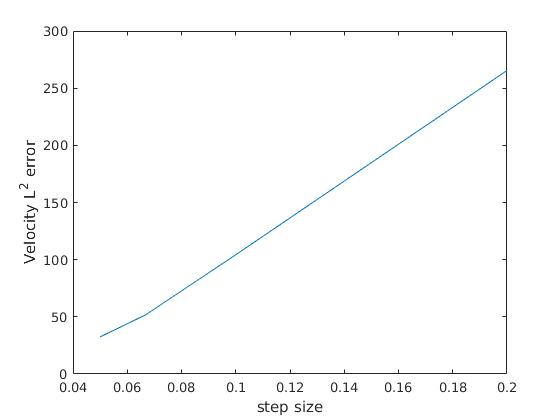
\includegraphics[width=\linewidth]{velocity_error_stokes.jpg}
  \caption{$h-$ convergence test for velocity in $L^2$ norm}
  \label{fig:vel_stoke_conv}
\end{figure}

\begin{figure}
  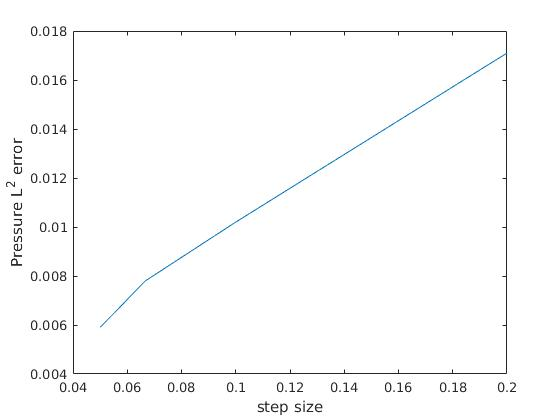
\includegraphics[width=\linewidth]{pressure_error_stokes.jpg}
  \caption{$h-$ convergence test for pressure in $L^2$ norm}
  \label{fig:pre_stoke_conv}
\end{figure}

We now present additional examples and check whether the implementation of Stokes flow is capable of reproducing physics of the problem.

\subsection{Lid-driven cavity problem}

We next present benchmark $CFD$ problem, Lid-driven cavity flow from \cite{Montlaur}. We solve the Stokes flow on Unit square [0,1] $\times$ [0,1] in $x-y$ plane. On boundaries ${x = 0}, {x = 1}$ and ${y = 0}$, we impose no slip or zero velocity dirichlet condition. On ${y = 1}$, we impose Dirichlet condition with Dirichlet velocity,

\begin{center}

\begin{equation}
u = (10x,0)^T \quad \textrm{for} \quad 0 \leq x \leq 0.1
\end{equation}

\begin{equation}
u = (1,0)^T \quad \textrm{for} \quad 0.1 \leq x \leq 0.9
\end{equation}

\begin{equation}
u = (10 - 10x,0)^T \quad \textrm{for} \quad 0.9 \leq x \leq 1
\end{equation}

\end{center}

The results are found to reproduce the physics of the problem. The plots of pressure are shown in figure \ref{fig:pressure_benchmark_stokes}, for $x-$velocity in figure \ref{fig:velocity_x_benchmark_stokes} and for $y-$velocity in figure \ref{velocity_y_benchmark_stokes}


\begin{figure}
  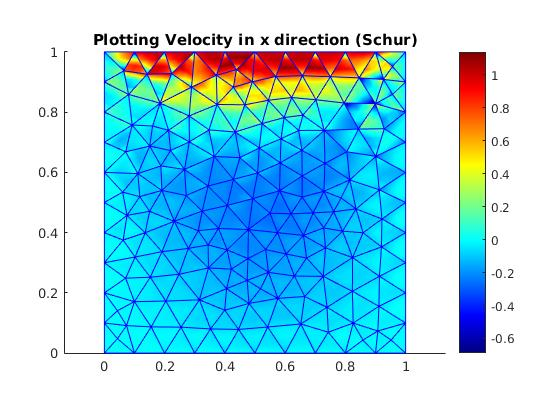
\includegraphics[width=\linewidth]{velocity_x_schur.jpg}
  \caption{x-velocity for Stokes flow for lid driven cavity problem}
  \label{fig:velocity_x_benchmark_stokes}
\end{figure}

\begin{figure}
  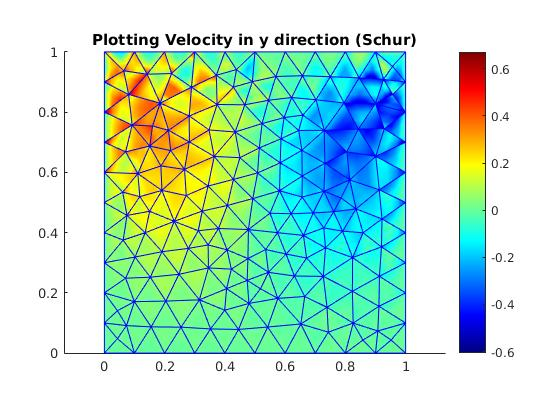
\includegraphics[width=\linewidth]{velocity_y_schur.jpg}
  \caption{y-velocity for Stokes flow for lid driven cavity problem}
  \label{fig:velocity_y_benchmark_stokes}
\end{figure}

\begin{figure}
  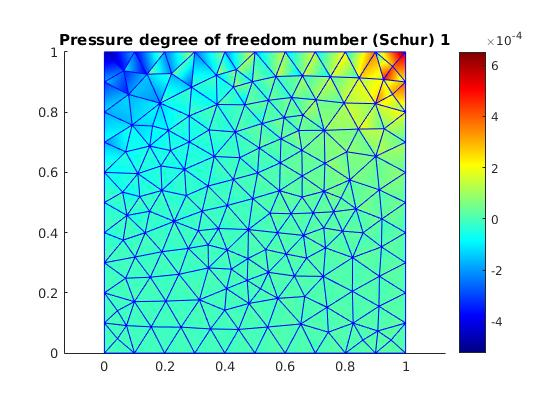
\includegraphics[width=\linewidth]{pressure.jpg}
  \caption{pressure for Stokes flow for lid driven cavity problem}
  \label{fig:pressure_benchmark_stokes}
\end{figure}

\subsection{Flow over cylinder}

The domain considered for this example is Unit square [0,1] $\times$ [0,1] in $x-y$ plane with cylinder of diameter 0.2 centered at $(0.5,0.5)$ i.e. the center of cylinder coincides with center of square. The boundary ${x=0}$ is dirichlet boundary with inflow velocity at point $(0,y)$ as $u = (y(1-y), 0)$. The boundaries ${y = 0}$ and ${y = 1}$ are Dirichlet boundaries with no slip or zero velocity condition. The boundary ${x = 1}$ is Neumann boundary with zero Neumann value i.e. $t = (0, 0)$. The source term is $f = (2 \nu - 1, 0)$. The results give physically relevant result for example, low pressure zone after cylinder, high pressure zone before cylinder and wake zone after cylinder for velocity.

The results are shown in figure \ref{fig:pressure_cylinder_stokes_minres} for pressure, figure \ref{fig:velocity_x_cylinder_stokes_minres} for $x-$velocity, \ref{fig:velocity_y_cylinder_stokes_minres} for $y-$velocity with solver $minres$ and in figure \ref{fig:pressure_cylinder_stokes_schur} for pressure, figure \ref{fig:velocity_x_cylinder_stokes_schur} for $x-$velocity, \ref{fig:velocity_y_cylinder_stokes_schur} for $y-$velocity with Schur complement method.

\begin{figure}
  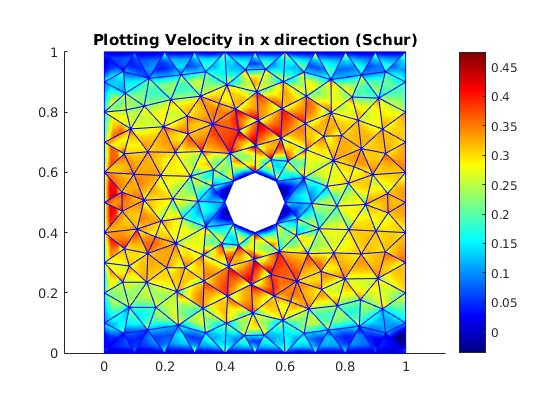
\includegraphics[width=\linewidth]{velocity_X_schur.jpg}
  \caption{$x-$velocity for Stokes flow for flow over cylinder (Schur complement)}
  \label{fig:velocity_x_cylinder_stokes_schur}
\end{figure}

\begin{figure}
  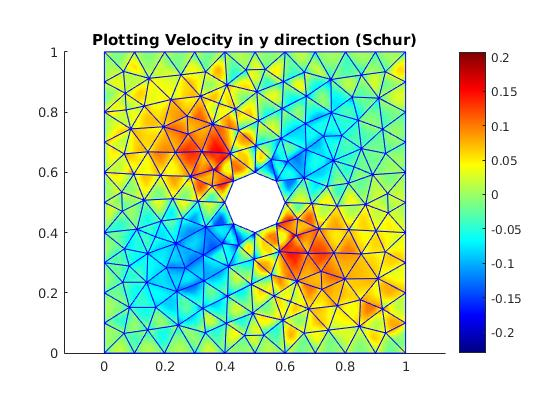
\includegraphics[width=\linewidth]{velocity_Y_schur.jpg}
  \caption{$y-$velocity for Stokes flow for flow over cylinder (Schur complement)}
  \label{fig:velocity_y_cylinder_stokes_schur}
\end{figure}

\begin{figure}
  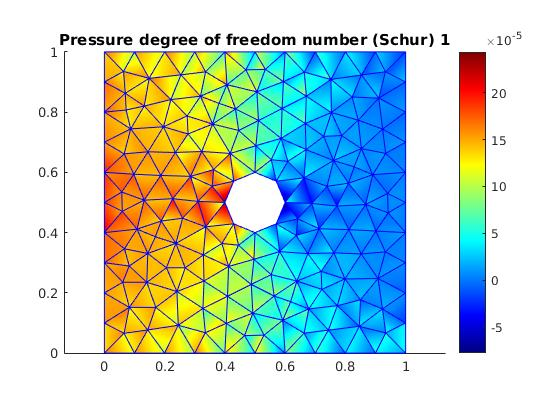
\includegraphics[width=\linewidth]{pressure_Schur.jpg}
  \caption{pressure for Stokes flow for flow over cylinder (Schur complement)}
  \label{fig:pressure_cylinder_stokes_schur}
\end{figure}

\begin{figure}
  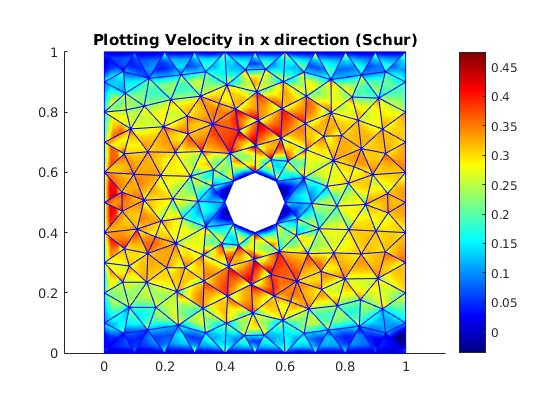
\includegraphics[width=\linewidth]{velocity_X_schur.jpg}
  \caption{$x-$velocity for Stokes flow for flow over cylinder (Schur complement)}
  \label{fig:velocity_x_cylinder_stokes_schur}
\end{figure}

\begin{figure}
  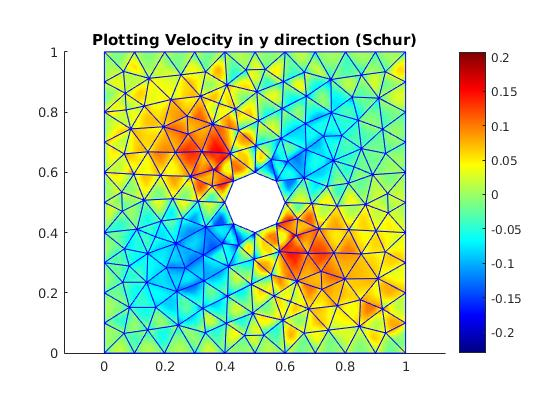
\includegraphics[width=\linewidth]{velocity_Y_schur.jpg}
  \caption{$y-$velocity for Stokes flow for flow over cylinder (Schur complement)}
  \label{fig:velocity_y_cylinder_stokes_schur}
\end{figure}

\begin{figure}
  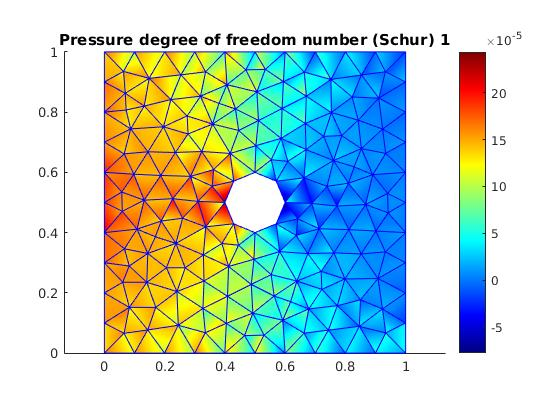
\includegraphics[width=\linewidth]{pressure_Schur.jpg}
  \caption{pressure for Stokes flow for flow over cylinder (Schur complement)}
  \label{fig:pressure_cylinder_stokes_schur}
\end{figure}

\section{Penalty parameter}

We now measure the effect of Penalty parameter on condition number of matrix. While coercivity provides lower limit for penalty parameter, the upper limit is based on affordable condition number of stiffness matrix. As shown in figure $vnjkvhjkhjkgh$, the condition number of stiffness matrix increases with increasing penalty parameter.
The condition number is measured on Unit square [0,1] $\times$ [0,1] in $x-y$ plane on $horizontal interval \times vertical interval$.

\begin{Huge}
Add figure here and cite figure above
\end{Huge}

\section{Selection of solver}

In order to solve variation form of Stokes equation we use Biconjugate gradients stabilized method popularly known as $bicgstab$, Minimum residual method better knwon as $minres$ and Schur complement method. The $bicgstab$ and $minres$ are in built solvers of MATLAB $howtociteMATLAB$. Schur complement method (Section \ref{schur}) is implemented separately based on Cholesky decomposition (Section \ref{chol}).

\subsection{Biconjugate gradients stabilized method}

The $bicgstab$ works to minimise residual of linear equation of the form:

\begin{equation} \label{linear_matrix_equation}
KX = B
\end{equation}

with $K$ = Coefficient matrix, $X$ = Vector of unknowns and $B$ = vector of value of known function. The coefficient matrix $A$ need not be symmetric. 

\begin{Huge}
Add working algorithm
\end{Huge}

In the present analysis it was found that the $bicgstab$ stops before converging to specified tolerance level or reaching maximum number of iterations. We expect that this is due to reaching a point which has zero Gradient but is not local optimal i.e. Saddle point formulation (Section \ref{saddle_point}). 

\subsection{Minimum residual method} 

The $minres$ method is special kind of Conjugate gradient method but does not require LU decomposition. It also solves the equations \ref{linear_matrix_equation}. However, the co-efficient matrix $K$ must be symmetric. 

\begin{Huge}
Add working algorithm
\end{Huge}

As the co-efficient matrix in case discrete form of Stokes equation is symmetric, the minres is suitable solver. Moreover, it has shown to coverge to required convergence level, provided sufficient number of iterations, when $bicgstab$ is not able to reach required level of convergence.

\subsection{Schur complement method} \cite{Fritzen} \label{schur}

We subdivide the matrix form of Stokes equation \eqref{Stokes_matrix} into smaller dimension system by Schur complement. We also note that matrix $A$ is symmetric positive definite and matrix $K$ is symmetric.
Here, $A \in \mathbb{R}^{ndofs\quad velocity \times ndofs \quad velocity}$; $B \in \mathbb{R}^{ndofs \quad velocity \times ndofs \quad pressure}$; $U,F_1 \in \mathbb{R}^{ndofs \quad velocity}$; $P, F_2 \in \mathbb{R}^{ndofs \quad pressure}$. \\

We solve equation \eqref{Stokes_matrix} in following steps,\\

STEP 1: \\ 
\begin{equation}\label{schur step 1}
U = A^{-1}(F_1 - BP) 
\end{equation}

The matrix $A$ is inverted by Cholesky decomposition (section \ref{chol}). 

STEP 2 : \\
We substitute now equation \eqref{schur step 1} into equation \eqref{continuity discrete} and \eqref{stokes discrete}.
\begin{equation}\label{schur step 2}
(0 - B^T A^{-1} B) P = F_2 - B^T A^{-1} F_1
\end{equation}

STEP 3 : \\
We now back substitute $P$ in equation \eqref{schur step 1} and compute $U$ in order to eventually obtain the solution vector.
\\

The success of this method primarily depends upon sparsity pattern of $B$ and efforts required for inverting $A$. The Cholesky decomposition provides faster approach for inverting $A$ due to symmetric positive definite nature of $A$. \\

In the present analysis, we find that Schur complement is much faster and in fact, for low flow velocities accurate method. Also Cholesky decoposition provides error message in case $A$ is not symmetric positive definite, indicating improper choice of penalty parameter. However, for high flow velocity this method is not very accurate. 

\section{Navier Stokes flow}

Stokes flow is an example of Navier Stokes flow with low Reynolds number, $Re$. In case of high Reynolds number the inertial force can no longer be neglected and hence we need to add inertial foces in Stokes flow. (We use the notations same as defined in section \ref{Stokes_flow}).

The strong form of Navier Stokes equation can be written as,

\begin{equation} \label{navier_stokes_strong}
-\nu \Delta u + \nabla p + (u \cdot \nabla) u = f \quad \textrm{in} \quad \Omega
\end{equation}

with Dirichlet and Neumann boundary condition as per section \ref{Stokes_flow}. Also the continuity equation as mentioned in section \ref{Stokes_flow} is valid.

The inertial forces term in weak form is as below,

\begin{equation}
\begin{split}
c(w;u,\phi) = \sum_{i=1}^{nel} \int_{\partial \Omega_i \setminus \Gamma_N} \frac{1}{2} [[(w \cdot n_i)(u^{ext} + u) - |w \cdot n_i|(u^{ext} - u)]] \cdot \phi \\ + \int_{\Gamma_N} (w\cdot n) u \cdot \phi -((w\cdot \nabla)\phi,u)
\end{split}
\end{equation}

Hence, the Navier Stokes equation can be written as,

\begin{equation}\label{navier_stokes_weak}
\begin{split}
a_{IP}(u,\phi) + c(u;u,\phi) + b(\phi,p) + (\{p\},[n\cdot \phi])_{\Gamma \cup \Gamma_D} = l_{IP}(\phi) 
\end{split}
\end{equation}

Here, we can see that the $c(u,u,\phi)$ is non linear term.

In discrete form this equation can be written as,

\begin{equation}
AU + C(U) U + BP = F
\end{equation} 

Here, $C(U)$ is a matrix which is dependent on solution vector $U$ and hence making the system of equation non linear.

In matrix form the Navier Stokes equation with Continuity equation can be written as,

\begin{equation} \label{Stokes_matrix}
\begin{spmatrix}{K}
    A+C(U) & B \\
    B^T & 0
\end{spmatrix}
\begin{spmatrix}{X}
    U \\
    P
\end{spmatrix}
=
\begin{spmatrix}{B}
    F_1  \\
    F_2
\end{spmatrix}
\end{equation}

\subsection{Newton method} \cite{Haasdonk} \label{newton_method}

We derive newton method for solving non linear system of equation arising out of discrete form of Navier Stokes equation. For $u, \phi , h \in \mathbb{V}$ and $p, \psi , h' \in \mathbb{Q}$ \\
\begin{equation}
S(u) = a(u,\phi) + b(\phi,p) + (\{p\},[n\cdot \phi])_{\Gamma \cup \Gamma_D} - l_{IP}(\phi)
\end{equation}


\begin{equation}
\begin{split}
S(u+h) - S(u) = (a(u+\delta h,\phi) + c(u + \delta h;u + \delta h,\phi)\\ + b(\phi,p+\delta h') + (\{p+\delta h'\},[n\cdot \phi])_{\Gamma \cup \Gamma_D} - l_{IP}(\phi)) - (a(u,\phi)\\ + c(u,u,\phi) + b(\phi,p) + (\{p\},[n\cdot \phi])_{\Gamma \cup \Gamma_D} - l_{IP}(\phi))
\end{split}
\end{equation}


\begin{equation}
\begin{split}
S(u+h) - S(u) = 2\delta c(u,h,\cdot) + \delta^2 c(h,h,\cdot) + \delta a(h,\cdot)\\ + \delta b(h',\cdot) + \delta (\{h'\},[n\cdot \phi])_{\Gamma \cup \Gamma_D}
\end{split}
\end{equation}


\begin{equation}
DS(u) = \lim_{\delta \to 0} \frac{S(u+h)-S(u)}{\delta}
\end{equation}

\begin{equation}
\begin{split}
DS(u) = 2 c(u,h,\cdot) + a(h,\cdot) + b(h',\cdot) + (\{h'\},[n\cdot \phi])_{\Gamma \cup \Gamma_D}
\end{split}
\end{equation}\\

Following similar procedure we write for continuity equation:\\
\begin{equation}
S'(u) = b(u,\psi) + (\{\psi\},[n \cdot u])_{\Gamma \cup \Gamma_D} - (\psi,n \cdot u_D)_{\Gamma_D}
\end{equation}

\begin{equation}
S'(u+\delta h) = b(u + \delta h,\psi) + (\{\psi\},[n \cdot u + \delta h])_{\Gamma \cup \Gamma_D} - (\psi,n \cdot u_D)_{\Gamma_D}
\end{equation}

\begin{equation}
DS'(u) = b(h,\psi) + (\{\psi\},[n \cdot \delta h])_{\Gamma \cup \Gamma_D} 
\end{equation}
\\
Algotrithm for the above newton method is as follow:\\

1. Select $u^k \in \mathbb{V}$ at iteration $k$\\

2. Verify $DS_{u^k}(h^k) = -S(u^k)$\\

3. Set $u^{k+1} := u^k + h^k$ till $||u^{k+1} - u^k|| < tol$ where $tol$ is specified tolerance.\\

In discrete form newton method means, solving the equation

\begin{equation} 
\begin{spmatrix}{K^k}
    A+C(U^k) & B \\
    B^T & 0
\end{spmatrix}
\begin{spmatrix}{X^{k+1}}
    U^{k+1} \\
    P
\end{spmatrix}
=
\begin{spmatrix}{B}
    F_1  \\
    F_2
\end{spmatrix}
\end{equation}

to reach convergence i.e. $||U^{k+1} - U^k|| < tol$

For success of Newton method it is important to have good initial guess. For Navier Stokes method we use solution of Stokes equation as initial guess.

\section{Sparsity pattern}

It is the connectivity of a node with neighbouring nodes that gives rise to different discontinuous Galerkin formulations. In general the flux terms are responsible for connecting to other nodes. This is also demonstrated in assembly process in chapter \ref{implementation_aspects}. We plot sparsity patterns of different matrices in figure $dvfzhvgfgv$.

\begin{huge}
Add figure here and cite figure above
\end{huge}

\section{Program flow}

\subsection{Grid Preparation}

We use $pdegrid$ tool to generate grid. We generate mesh and export parameters $point(p)$, $edge(e)$ and $triangle(t)$. $params.bnd\_rect\_corner1$ marks the lower corner of to be marked boundary and $params.bnd\_rect\_corner2$ marks the upper corner of to be marked boundary. $params.bnd\_rect\_index$ marks the type of boundary. $-1$ represents Dirichlet boundary and $-2$ represents Neumann boundary. $params.gridtype$ defines the type of grid. $construct\_grid(params)$ constructs the grid as struct containing necessary fields for grid. 

In case of creating rectangular grid without using $pdegrid$, we define fields $xrange$, $yrange$, $xnumintervals$ and $ynumintervals$ defining range of x co-ordinates of domain, range of y co-ordinates of domain, number of intervals for x division and number of intervals for y division respectively and call routine $construct\_grid$.

\subsection{Function space formulation}

We now define fields for constructing function spaces for pressure and velocity. We define now two structures $params$ for velocity and $paramsP$ for pressure. These structures contain fields (as relevant to function space formulation) $pdeg$ and $dimrange$. $pdeg$ represents polynomial degree of Ansatz function and $dimrange$ represents  dimension of qunatity i.e. 2 for velocity and 1 for pressure. The field $paramsP.pdeg$ is calculated as $paramsP.pdeg = params.pdeg - 1$ in accordance with Taylor hood element. Based on these fields $ndofs\_per\_element$, $ndofs$ are calculated. Number of elements in grid can be read from $grid.nelements$. We also define degree for integration $qdeg$ and kinematic viscocity in $params.kinematic\_viscosity$. Variable $mu$ also holds the value of kinematic viscocity. we define penalty parameter in variable $C11$. $show\_sparsity$ is the field used to plot sparsity pattern of each matrix if set to true.\\

\subsection{Matrix assembly}

We now assemble all the matrices as explained in chapter \ref{implementation_aspects}. \\$params.bilinear\_side$ contains $A$ or assembly of $a(u,\phi)$\\$params.bilinear\_side\_pressure\_terms$ contains assembly of $B$ or assembly of $b(\phi,\psi)$\\ $params.lhs\_continuity$ contains assembly of $B^T$\\ $rhs$ is the right hand side matrix $[F_1;F_2]$ as\\ $[params.linear\_side;params.rhs\_continuity]$. \\

\subsection{Solving assembled form}

We now define the solver specific variables. $required\_residual\_tol$ specifies the required accuracy from solver in solution and $max\_iter$ specifies the maximum number of iterations that is used to stop the solver in case the solver does not converge. We call the routine $solve\_plot\_solution$ for $bicgstab$,$minres$ (The solver is specified in $solve\_plot\_solution$). In case of Schur complement method, routine $solve\_plot\_solution\_schur$ is used. The output variable $achieved\_residual\_tol$ contains residual value, $params$ and $paramsP$ are given new values $dofs$ which contain degree of freedom. $actual\_iter$ is the value of number of iterations at the end of iterations process. $flag$ specifies the criteria for end of iteration process.\\

\subsection{Post processing}

We now enter into $stifness\_matrix\_test$, explained in section \ref{Stokes_flow}. Then we enter into error measurement which measures the error in $L^2$ or $H_0$ norm. $params.dof\_analytical$, $paramsP.dof\_analytical$ contain analytical expression against which numerical solution is to be compared. $params.dof\_derivative\_analytical$ and  $paramsP.dof\_derivative\_analytical$ contain anlytical exprression for derivative to be used for $H_0$ norm.\\

\subsection{Newton method}

We now enter into newton method $newton\_script$. We define again solver specific variables $tol\_newton$, $max\_iter\_newton$, $tol_solver$, $max\_iter\_solver$. $tol\_newton$, $max\_iter\_newton$ are variables for ending newton method and $tol_solver$, $max\_iter\_solver$ are variables for solver to solve $h^k$ in each newton loop. We again measure the error in $L^2$ and $H_0$ norm.\\

\subsection{Additional remarks}

We plot the solution using  $ldg\_plot$ written for plotting discontinuous functions. The Dirichlet values are defined in $dirichlet\_values$, the Neumann values are defined in $neumann\_values$ and source function is defined in $func\_rhs$. 

\chapter{Appendix}

\section{List of symbols} \label{symbol_list}

$w_i$ = Weight at corressponding point\\
$nop$ = Number of points\\
$h_\tau$ Diameter of element $\tau$\\
$\mathcal{T}$ Discretised domain\\
$\theta$ Smallest angle in all triangles $\tau \in \mathcal{T}$\\
$r$ Point in the triangular element\\
$r_1,r_2,r_3$ Vertices of triangular element\\
$\lambda_1, \lambda_2, \lambda_3$ Weights for Barycentric coordinates\\
$\mathbb{V}_h$ Truth space for Velocity\\
$\mathbb{Q}_h$ Truthe space for Pressure\\
$N_h$ Dimension of Truth space\\
$F_k$ Local to global coordinate system mapping\\
$a_{IP}, b, c$ Terms in weak formulation of Navier Stoks equation (Equation \eqref{navier_stokes_weak_ch3}) \\
$A,B,C$ Matrix terms in corressponding to $a_{IP}, b, c$\\
$U$ Velocity solution vector \\
$P$ Pressure solution vector\\
$F_1,F_2$ Discrete form of right hand side of equation \eqref{navier_stokes_weak_ch3} and \eqref{contiuity_weak_ch3}\\
$g$ Function in global coordinate\\
$D$ Polynomial degree \\
$\phi$ Velocity basis function\\
$\hat{\phi}$ Velocity basis function on reference triangle\\
$\psi$ Pressure basis function\\
$\hat{\psi}$ Pressure basis function on reference triangle\\
$u$ Velocity unless specified otherwise\\
$p$ Pressure unless specified otherwise\\
$P$ Momentum of fluid flowing thorugh control volume\\
$cv$ Control volume\\
$cs$ Control system\\
$e$ Edge between two elements\\ 
$f$ Source/Sink/External force per unit volume\\
$F$ External force acting on $cv$\\
$\sigma$ Stress\\
$u_D$ Velocity at Dirichlet boundary\\
$\Gamma, \Gamma_D, \Gamma_N$ Interelemental/internal boundary, Dirichlet boundary, Neumann boundary respectively\\
$\tau$ Triangular grid element\\
$JIT$ Jacobian Inverse Transpose\\
$n$ Unit normal to an edge pointing outwards from the element\\
$\Omega$ Continuous domain\\
$\partial \Omega$ Continuous domain boundary\\
$\hat{T}$ Reference Triangle\\
$P^D$ Polynomial of degree at most $D$ over $\Omega$\\
$C_{11}$ Coercivity constant\\
$\gamma$ Continuity constant\\
$\beta$ Inf-sup constant\\
$\nu$ Kinematic viscocity\\
$B'$ Extensive property under consideration  \\
$b'$ Intensive property corressponding to B \\
$\rho$ Density of fluid \\
$t$ Neumann value\\
$t'$ time\\
$J_k$ Jacobian matrix of element $k$ or Rotational matrix for transformation from local co-ordinate system to global co-ordinate system\\
$C$ Translational vector for transformation from local coordinate system to global coordinate system\\
$X$ Coordinates of vertices of element in Global coordinate system\\
$\hat{X}$ Coordinates of vertices of reference triangle in local co-ordinate system\\
$L$ Characteristic length for Reynolds number\\
$\kappa_E$\\
$CFD$ Computational Fluid Dynamics\\
$bicgstab$ Biconjugate gradients stabilized method\\
$minres$ Minimum residual method\\

\section{Mathematical preliminaries}

\subsection{Cholesky decomposition} \label{chol}

Every symmetric Positive Definite Matrix can be expressed as product of Lower Triangular and transpose of that Lower Triangular Matrix. That is, if $U$ is symmetric positive definite matrix then,

\begin{equation}
U = LL^T
\end{equation}

where, $L$ is lower triangular matrix. It is to be noted that $L^T$ is an upper triangular matrix. \\

Cholesky decomposition is useful especially when inverting an Matrix in MATLAB. Since the back division operator ($\setminus$) recognises the lower triangular structure of matrix, it proceeds with division process.\\

We now explain the algorithm for Cholesky decomposition. \\

\begin{equation} \label{Stokes_matrix}
\begin{spmatrix}{U}
    a_{11} & a_{12} & a_{13}\\
    a_{21} & a_{22} & a_{23}\\
    a_{31} & a_{32} & a_{33}\\
\end{spmatrix}
=
\begin{spmatrix}{L}
    l_{11} & 0 & 0\\
    l_{21} & l_{22} & 0\\
    l_{31} & l_{32} & l_{33}
\end{spmatrix}
\begin{spmatrix}{L^T}
    l_{11} & l_{21} & l_{31}\\
    0 & l_{22} & l_{32}\\
    0 & 0 & l_{33}
\end{spmatrix}
\end{equation}

We see that,\\
\begin{equation}
a_{11} = l_{11}^2, \quad a_{22} = l_{21}^2 + l_{22}^2, \quad a_{33} = l_{31}^2 + l_{32}^2 + l_{33}^2
\end{equation}

and 
\begin{equation}
a_{12} = a_{21} = l_{11}l_{21}, \quad a_{13} = a_{31} = l_{11}l_{31}, \quad a_{23} = a_{32} = l_{31}l_{21} + l_{32}l_{22}
\end{equation}

We now see that for diagonal elements,\\

\begin{equation}
l_{kk} = \sqrt{a_{kk} - \sum_{k=1}^{j-1} l_{kj}^2}
\end{equation}

and for elements below diagonal,\\

\begin{equation}
l_{ik} = \frac{1}{l_{kk}}(a_{ik}-\sum_{j=1}^{k-1} l_{ij}l_{kj})
\end{equation}
\\
It is to be noted that similar theory is also applicable for Cholesky decomposition with upper triangular matrix instead of lower triangular matrix. Also, this algorithm can be extended to Matrix of any size. \\

In MATLAB the cholesky decomposition is performed by $chol$. The choice of upper triangular or lower triangular matrix can be adjusted by providing additional input argument $'lower'$ or $'upper'$. More information can be found by $help$ in MATLAB and MATLAB documentation.
 
\subsection{Saddle point formulation} \label{saddle_point} \cite{saddle}

The saddle point problem has following form,

\begin{equation} 
\begin{spmatrix}{}
    A & B_1 \\
    B_2 & C
\end{spmatrix}
\begin{spmatrix}{}
    X \\
    Y
\end{spmatrix}
=
\begin{spmatrix}{}
    f  \\
   	g
\end{spmatrix}
\end{equation}

\begin{equation}
A \in \mathbb{R}^{n \times n}; B_1, B_2 \in \mathbb{R}^{m \times n}; C \in \mathbb{R}^{m \times m} 
\end{equation}

with $n \geq m$.\\

We assume here that $A, B_1, B_2$ are non zeros. Usually constituents $A,B,C$ satisfy one or more of following properties.
\\
\\
1. $A = A^T$ (Symmetric)\\
2. Symmetric part of $A$ is positive semi definite\\
3. $B_1 = B_2 = B$\\
4. $C$ is symmetric and positive semidefinite\\
5. $C = 0$ (Zero matrix)\\

Incompressible Stokes equation is an example of Saddle point problem with $A$ being symmetric positive definite matrix, $B_2 = B_1^T$ and $C = 0$. \\

\textbf{Remarks}:\\

1. Saddle point problem has points with zero slope but not local optimum.\\

1. In case $A$ is symmetric positive definite the Schur complement is very useful method.\\

2. In general not much can be said about the eigen values of Saddle point matrix.\\ 

3. Saddle point systems obtained in practical problems can be poorly conditioned.\\

4. Also number of methods such as Krylov subspace methods, Multilevel methods have been developed for saddle point problems.\\

\subsection{Basic definitions}\cite{crbm}

Let $\mathbb{V}$ be a vector space over $\mathbb{R}$

1. For a set $\lbrace w_1,....,w_N \rbrace \subset \mathbb{V}$ we denote by \\
\begin{equation} \label{vector space}
\mathrm{span} \lbrace w_1,....,w_2 \rbrace = \lbrace v \in \mathbb{V} | v = \Sigma_{n=1}^N \alpha_n w_n, \alpha_n \in \mathbb{R} \rbrace
\end{equation} 

the linear subspace spanned by the elements $w_1,....,w_N$.\\

2. The space $\mathbb{V}$ is of finite dimension if there exists a maximal a set of linearly independent elements $v_1,....,v_N$, otherwise $\mathbb{V}$ is of infinite dimension.\\

3. A norm $||.||_\mathbb{V}$ on $\mathbb{V}$ is a function $||.||_\mathbb{V} : \mathbb{V} \rightarrow \mathbb{R}$ such that\\ 
A. $||v||_\mathbb{V} \geq 0 \forall v \in \mathbb{V}$ and $||v||_\mathbb{V} = 0$ iff $v=0$\\
B. $||\alpha v||_\mathbb{V} = |\alpha| ||v||_\mathbb{V}$  $\forall \alpha \in \mathbb{R}, v \in \mathbb{V}$\\
C. $||u+v|| \leq ||u||_\mathbb{V} + ||v||_\mathbb{V}$\\

4. The pair $(\mathbb{V},||.||_\mathbb{V})$ is a normed space and we can define a distance function $d(u,v) = ||u-v||_\mathbb{V}$ to measure the distance between two elements $u,v \in \mathbb{V}$.\\

5. A semi-norm on $\mathbb{V}$ is a function $|.|_\mathbb{V} : \mathbb{V} \rightarrow \mathbb{R}$ such that $|v|_\mathbb{V} \geq 0$ for all $v \in \mathbb{V}$ and B. and C. above are satisfied. In consequence a semi-norm is a norm iff $|v|_\mathbb{V} = 0$ implies  $v = 0$.\\

6. Two norms $||.||_1$ and $||.||_2$ are equivalent if there exists two constants $C_1,C_2 > 0$ such that \\

\begin{equation} \label{norm_equivalent}
C_1||.||_1 \leq ||.||_2 \leq C_2 ||.||_1 \forall v \in V
\end{equation}

\subsection{Linear forms}

Let $(\mathbb{V,||.||_\mathbb{V}})$ be a normed space. Then, we define the following notions.\\

1. A function $F : \mathbb{V} \rightarrow \mathbb{R}$ is said to be linear, a $functional$ or a $linear form$ if  \\

\begin{equation} 
F(u+v) = F(u) + F(v) \forall u,v \in \mathbb{V} 
\end{equation}

\begin{equation} 
F(\alpha u) = \alpha F(u) \forall \alpha \in \mathbb{R}, u \in \mathbb{V}
\end{equation}

2. F is $bounded$ if there exists a constant $C > 0$ such that\\ 
\begin{equation} 
|F(v)| \leq C ||v||_\mathbb{V} \forall v \in \mathbb{V}
\end{equation}

3. F is $continuous$ if for all $\epsilon > 0$ there exists a $\delta_\epsilon > 0$ such that \\
\begin{equation}
||u - v||_\mathbb{V} \leq \delta_\epsilon \Rightarrow  |F(u) - F(v)| < \epsilon
\end{equation}

The notion of continuity and boundedness is equivalent for linear forms.

\subsection{Bilinear forms}

1. A bilinear form $a(\cdot,\cdot)$ acting on the vector spaces $\mathbb{V}$ and $\mathbb{W}$ is given as\\
\begin{equation}
a : \mathbb{V} \times \mathbb{W} \Rightarrow \mathbb{R}
\end{equation}

\begin{equation}
(u,v) \mapsto a(u,v)
\end{equation}

and is linear with respect to each of its arguments.\\

2. Let $\mathbb{V}$ and $\mathbb{W}$ be endowed with the norms $||\cdot||_\mathbb{V}$ and $||\cdot||_\mathbb{W}$. A bilinear form $a(\cdot,\cdot)$ is continuous if there exists a constant $\gamma > 0$ such that,\\
\begin{equation}
|a(\cdot,\cdot)| \leq \gamma ||u||_\mathbb{V} ||v||_\mathbb{W} \forall u,v \in \mathbb{V}
\end{equation}

3. If $\mathbb{V} = \mathbb{W}$, a bilinear form $a(\cdot,\cdot)$ is $coercive$ if there exists a constant $\alpha > 0$ such that \\
\begin{equation}
a(v,v) \geq \alpha ||v||_\mathbb{V}^2 \forall v \in \mathbb{V}
\end{equation}

\section{Coercivity of bilinear form} 

For the term $a_{IP}$ which has elliptic behavior we discuss now coercivity, continuity and inf-sup condition\cite{riviere}.

A bilinear form $a(u,v)$ is said to be coercive if there exists a constant $c_{11} > 0$ such that

\begin{equation}\label{Coercivity}
a(v,v) > c_{11} ||v||^2   \exists   c_{11} > 0
\end{equation}

Based on \ref{basics}

\begin{equation}\label{Coercivity_constant}
a(v,v) \geq (1-\frac{\delta}{2} |1-\epsilon|) \Sigma_{E \epsilon \varepsilon_h} ||\nu^{1/2} \nabla v ||^2_{L^2(E)} + \Sigma_{e \epsilon \Gamma_h \cup \Gamma_D} \frac{\sigma_e^0 - \frac{C_t^2 \nu_1^2 n_0}{2 \delta K_0}|1-\epsilon|}{|e|^{\beta_0}} ||[v]||^2_{L^2(e)}
\end{equation}

\section{Continuity of bilinear form}

A bilinear form $a_{IP}(u,v)$ is said to be continuous if there exists a constant $\gamma > 0$ such that

\begin{equation}\label{Continuity_constant}
a_{IP}(u,v) \leq \gamma ||u||||v||   \exists   \gamma > 0
\end{equation}


\subsection{Coercivity constant for equation for Stokes flow} \label{basics}

We define a lower and upper bound for the viscosity such that \\
\begin{equation}
\nu_0 \leq \nu \leq \nu_1
\end{equation}

Using Cauchy Schwarz inequality

$\Sigma_{e \epsilon \Gamma_h \cup \Gamma_D} \int_e {\nu}[n\otimes \phi] \leq \Sigma_{e \epsilon \Gamma_h \cup \Gamma_D} ||\nu \nabla \phi \cdot n||_{L^2(e)} ||[\phi]||_{L^2(e)} \leq \Sigma_{e \epsilon \Gamma_h \cup \Gamma_D} ||\nu \nabla \phi \cdot n||_{L^2(e)} {\frac{1}{|e|}}^{(1/2-1/2)} ||[\phi]||_{L^2(e)}$

Based on the Trace inequatlity and the lower and upper bound for viscocity, for neighbouring elements $E_1^e$ and $E_2^e$ sharing the edge $e$ 
\begin{equation}
||{\nu \nabla \phi \cdot n}||_{L^2(e)} \leq \frac{C_t \nu_1}{2} {h_{E_1^e}}^{-1/2} ||\nabla \phi||_{L^2(E_1^e)} + \frac{C_t \nu_1}{2} {h_{E_2^e}}^{-1/2} ||\nabla \phi||_{L^2(E_2^e)}
\end{equation}

where $h_E$ is the diameter of element E.

Again based on the trace inequality

\begin{equation}
\int_e {\nu \nabla \phi}[n \otimes \phi] \leq (\frac{C_t \nu_1}{2} {h_{E_1^e}}^{-1/2} ||\nabla \phi||_{L^2(E_1^e)} + \frac{C_t \nu_1}{2} {h_{E_2^e}}^{-1/2} ||\nabla \phi||_{L^2(E_2^e)}) |e|^{\beta_0/2} {1/|e|}^{\beta_0/2} ||[\phi]||_{L^2(e)}
\end{equation}

For $h \leq 1$ and the $\beta_0 (d-1) \geq 1$ we obtain a similar bound for the boundary edges.

If $n_0$ denotes maximum number of neighbours $n_0 = 3$ for triangles,
\begin{equation}
\int_e {\nu \nabla \phi}[n \otimes \phi] \leq C_t \nu_1 (\Sigma_{e \ epsilon \Gamma_h \cup \Gamma_D} \frac{1}{|e|^\beta_0} ||[\phi]||^2_{L^2(e)})^(1/2) \times (\Sigma_{e \epsilon \Gamma_h} ||\nabla \phi||^2_{L^2(E_1^e)} + ||\nabla \phi||^2_{L^2(E_1^e)} + \Sigma_{e \epsilon \Gamma_D} ||\nabla \phi||^2_{0,E_1^e})
\end{equation}

Using Young's inequality for $\delta > 0$

\begin{equation}
\int_e {\nu \nabla \phi}[n \otimes \phi] \leq \frac{\delta}{2} \Sigma_{E \epsilon \varepsilon_h} ||\nu^{1/2} \nabla v ||^2_{L^2(E)} +  \frac{C_t^2 \nu_1^2 n_0}{2 \delta K_0} \frac{1}{|e|^{\beta_0}} ||[v]||^2_{L^2(e)}
\end{equation}


Substituting this in bilinear form we arrive at the result in \ref{Coercivity_constant}.

\subsection{Sobolev spaces} \cite{crbm}

Let $\Omega$ be an open subset of $\mathbb{R}^d$ and $k$ a positive integer. Let $L^2(\Omega)$ denote the space of square integrable functions on $\Omega$. 

1. The \textit{Sobolev space of order k} on $\Omega$ is defined by\\
\begin{equation}
H^k (\Omega) = \lbrace f \in L^2 (\Omega) | D^\alpha f \in L^2 (\Omega), |\alpha| \leq k \rbrace ,
\end{equation} 

where $D^\alpha$ is the partial derivative
\begin{equation}
D^\alpha = \frac{\partial^{|\alpha|}}{\partial x_d^{\alpha_1} ..... \partial x_d^{\alpha_d}}
\end{equation}

in the sense of distributions for the multi-index $\alpha = (\alpha_1,.....,\alpha_d) \epsilon \mathbb{N}^d$ using the notation $|\alpha| = \alpha_1 + ..... + \alpha_d $.

It holds by construction that $H^{k+1}(\Omega) \subset H^k (\Omega)$ and that $H^0 (\Omega) = L^2 (\Omega)$. $H^k(\Omega)$ is a Hilbert space with the inner product
\begin{equation}
(f,g)_{H^k(\Omega)} = \Sigma_{\alpha \epsilon \mathbb{N}^d, |\alpha| \leq k} \int_\Omega (D^\alpha f) (D^\alpha g)
\end{equation}

and the induced norm 

\begin{equation}
||f||_{H^k (\Omega)} = \sqrt{(f,f)_{H^k(\Omega)}} = \sqrt{\Sigma_{\alpha \epsilon \mathbb{N}^d, |\alpha| \leq k} \int_\Omega |D^\alpha f|^2}
\end{equation}

and the semi norm 

\begin{equation}
||f||_{H^k (\Omega)} = \sqrt{\Sigma_{\alpha \epsilon \mathbb{N}^d, |\alpha| = k} \int_\Omega |D^\alpha f|^2}
\end{equation}

In case of the discontinuous Galerkin space we use the broken Sobolev norm (for symmetric interior penalty Galerkin), \cite{Montlaur2}

\begin{equation}
||f||_{1,h}^2 = \Sigma_{K \epsilon \tau_h} ||\nabla f||_{L^2(K)}^2 + \Sigma_{E \epsilon \varepsilon(\tau_h)} \kappa_E \nu ||[[u]]||_{L^2 (E)}^2
\end{equation}

and inner product \\

\begin{equation}
(f,g) = \Sigma_{K \in \tau_h} (f,g)_{L^2(K)} + \Sigma_{E \in \varepsilon(\tau_h)} \kappa_E \nu ([u],[v])_{L^2 (E)}
\end{equation}


\subsection{Trace theorem} \cite{riviere}

The trace inequalities are used to define restrictions of Sobolev function along the boundary of domain. These inequalities are used for proper treatment of Boundary conditions. These conditions are stated below:

$\forall \phi \epsilon \mathbb{P}_k(\tau)$, $\forall \Gamma \subset \partial \Omega$

if $e$ is the length of $\Gamma$ and $E$ is the area of $\tau$

\begin{equation}
||\phi||_{L^2(\Gamma)} \leq \hat{C}_t |e|^{\frac{1}{2}} |E|^{\frac{-1}{2}} ||\phi||_{L^2(\tau)}
\end{equation}

\begin{equation}
||\phi||_{L^2(\Gamma)} \leq {C}_t |h_E|^{\frac{-1}{2}} ||\phi||_{L^2(\tau)}
\end{equation}

\begin{equation}
||\nabla \phi \cdot n||_{L^2(\Gamma)} \leq \hat{C}_t |e|^{\frac{1}{2}} |E|^{\frac{-1}{2}} ||\nabla \phi||_{L^2(\tau)}
\end{equation}

\begin{equation}
||\nabla \phi \cdot n||_{L^2(\Gamma)} \leq {C}_t |h_E|^{\frac{-1}{2}} ||\nabla \phi||_{L^2(\tau)}
\end{equation}

Here, $\hat{C}_t$ and ${C}_t$ are constants independent of $h_E$ and $\phi$ but depenedent on polynomial degree $k$.

The exact expressions for $C_t$ can be obtained from \cite{warburton}.

\subsection{Cauchy-Schwarz and Young's inequality}\cite{riviere}

Cauchy-Schwarz inequality,\\
\begin{center}
$\forall f,g \epsilon L^2(\Omega)$, $|(f,g)_{\Omega}| \leq ||f||_{L^2(\Omega)} ||g||_{L^2(\Omega)}$ \\
\end{center}

Young's inequality,\\
\begin{center}
$\forall \epsilon > 0$, $\forall a,b \epsilon \mathbb{R}$, $ab \leq \frac{\epsilon}{2}a^2 + \frac{1}{2 \epsilon}b^2$\\
\end{center}

\bibliographystyle{plain}
\bibliography{ref1}

\end{document}